\clearpage
\section{Architectural Design}
\subsection{Overview}
\subsubsection{High Level View}
The CKB application is a distributed system that guarantees fault tolerance, availability, reliability, and performance, built on the concept of microservices. A microservices architecture is a type of application architecture where the application is developed as a collection of services, which are units of functionalities designed to support interoperable machine-to-machine interaction over a network. A representation of the system, as described, is available in Figure 1. \par

The choice of this architectural style is due to many factors, including:

\begin{itemize}
    \item \textit{Scalability}: Microservices can be scaled independently, allowing for scaling out sub-services without scaling out the entire system. This leads to the versatility of the application.
    
    \item \textit{Fault Tolerance}: Unlike the monolithic approach, which has many inter-dependencies creating a single point of failure, in this approach, the application can remain mostly unaffected by the failure of a single module.
    
    \item \textit{Deployment and Productivity}: Microservices enable continuous integration and delivery, making it easy to test new ideas, suiting Agile and DevOps working methodologies. Furthermore, it makes it easier to split the work between team members: each team member is responsible for a particular service, resulting in a smart, productive, cross-functional team where the speed of development is largely improved.
    
    \item \textit{Continuous Delivery}: Microservices enable continuous delivery, meaning your software can be modified and delivered to your client base frequently and easily due to its automated nature.
    
    \item \textit{Maintainability}: Benefits of Microservices Architecture include less energy spent on understanding separate pieces of software or worrying about how a bug fix will affect other parts of the product.
\end{itemize}

In detail, there are six microservices in the CKB application, described as follows:

\begin{itemize}
    \item \textbf{User Management Microservice}: This is the microservice to which every first request by a Web Client is forwarded. In order to grant high availability, this module is duplicated over various servers handling the requests. Its role is to grant access to the application. In doing so, it communicates with the GitHub Integration Microservice. Moreover, the module is in charge of displaying the home page, and so it communicates with the Tournament Microservice to obtain useful data for the user who just logged in. Every notification is obtained from the Notification Microservice, both synchronously (requesting directly) and asynchronously. For this reason, it needs to communicate with this module too.
    
    \item \textbf{Tournament Microservice}: This microservice grants control over the tournaments, involving score computation mechanisms and badge management too. In order to show the battles it is related to, it must communicate with the Battle Microservice. To grant the correct management of notifications, it communicates with the Notification Microservice.
    
    \item \textbf{Battle Microservice}: This is the microservice responsible for managing the battles. It communicates with the Notification Microservice to handle notifications addressed to it and with the Tournament Microservice, sending rankings and other important data to share. To guarantee the correct aim of the application, it needs to contact the GitHub Integration Microservice (e.g., when creating a new battle or when pushing code). Finally, it is interesting its communication with the Score Computation Microservice: sending data from a specific battle, doing so it could obtain the rankings.
    
    \item \textbf{GitHub Integration Microservice}: This microservice is in charge of handling all the API requests involving GitHub. To do this, it communicates with the Battle Microservice when it needs to share important information regarding the battles.
    
    \item \textbf{Score Computation Microservice}: The scope of this microservice is to calculate the rankings of the battles, managing the manual evaluation and the automatic testing of the code pushed by the user participating in the battle.
    
    \item \textbf{Notification Microservice}: This microservice is useful for managing all the notifications involving tournaments and battles, sending them asynchronously (without an explicit request) to the users. This is the reason why it needs to communicate with the User Management Microservice.
\end{itemize}

This section is aimed to give an overview of the architectural elements composing the CodeKata system and their interaction. It contains also a detailed description of all the choices made for guarantee the strengths described in the RASD, such as reliability, security and availability.
\subsubsection{Distributed View}
\subsection{Component View}
This section aims at illustrating the various components that make up the \app system. In the following, UML Component diagrams are employed to illustrate the logical software elements that collaborate in order to achieve the goals set for the system to be developed.

Since the structure of components of the \app system wouldn't fit into a single diagram, multiple representations are supplied to make the document as clear as possible and avoid cluttering. 
The decisions regarding how to divide the diagrams of the Component View have been taken based on the idea of grouping together components that frequently interact with each other. 
It is important to mention that although the explanation makes use of separated graphics, the system is a single one and the elements represented here in different diagrams will be part of the same system and will take part in the overall functioning of the platform together.

\subsubsection{RESTful APIs component diagram}
\begin{minipage}{\linewidth}
One of the first characteristics that have been mentioned in the introductory section about \app is that microservices expose RESTful APIs in order to receive and respond to commands, expose data and collaborate with one another. This view aims at describing from a high perspective the ways microservices exploit these APIs to work.

\vspace*{1.5cm}
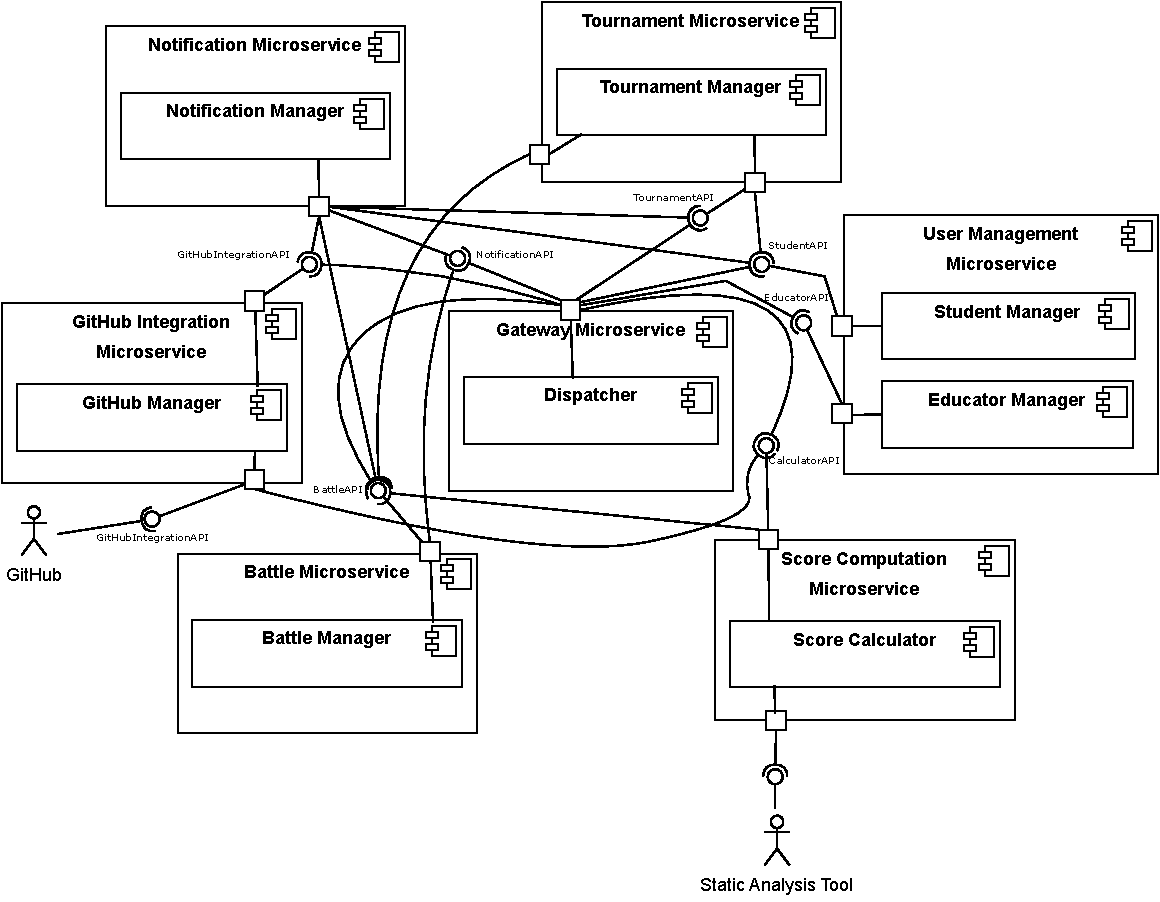
\includegraphics[width=\linewidth]{1Component_REST_API}

\end{minipage}

Let's break down the main ideas that the diagram tries to convey.
This UML component diagram is employed in order to show the RESTful APIs that are offered by each microservice in the system. These APIs provide specific computations on data related to the service offered by the microservice in question. For instance, the Tournament Microservice will expose an API that works on the tournaments data inside the shared database and exposes relevant information on tournaments.

The gateway is the entry point for all users’ requests. The Dispatcher component inside the Gateway is responsible for delivering the users' requests to the correct microservices that will have to handle them. This is why the Dispatcher "uses" all the APIs exposed by the other microservices. 

For some kinds of computations, the various microservices that compose \app may also exploit each other through their RESTful APIs. In this diagram, these interactions are shown. 
For instance:
\begin{itemize}
	\item The Notification Manager needs to query the Tournament manager and the Battle manager every time it has to retrieve the list of students subscribed to a tournament or to a battle (in order to deliver the notification to a specific set of students).
	\item The Notification Manager has to query the Student Manager when the list of all students of CodeKataBattle is needed (for example to notify all students of a new tournament available on the platform).
	\item The Notification Manager requires access to the data handled by the GitHub Manager in order to retrieve the link to the remote repository of a battle and compose the notification for all students subscribed to that battle (when the registration deadline of the battle passes).
	\item The GitHub manager component uses the CalculatorAPI in order to pass the downloaded source code of a new student solution to the Score Calculator component that will in turn automatically compute the score to assign to it.
	\item The Score Calculator must exploit the BattleAPI in order to request an update on the battle ranking every time a new score is available.
	\item The Tournament Manager requires access to the Student Manager data in order to assign badges when the tournament is closed.
\end{itemize}

This diagram has to be read and interpreted also accounting for the event-driven paradigm that is adopted in the project. Some of the interactions and flows of events inside the system happen in an asynchronous manner with an event-driven approach that is further described in the following views. That's why some interactions, that might seem missing here are actually handled in an asynchronous way to increase the performance of the overall system.

\subsubsection{Service Discovery component diagram}

\begin{minipage}{\linewidth}
	
	This very simple component diagram shows an important service that is offered by the Gateway microservice to allow all microservices to locate each other and therefore collaborate. This service is called "Service Discovery" and it consists in maintaining a register (inside the Gateway microservice) of active microservices. 
	
	In this way:
	\begin{itemize}
		\item A new microservice brought up can register itself in order to be localized by the other microservices.
		\item All microservices can contact other active microservices in the system to advance some requests.
	\end{itemize}
	
	Here's the diagram:
	
	\vspace{2cm}
	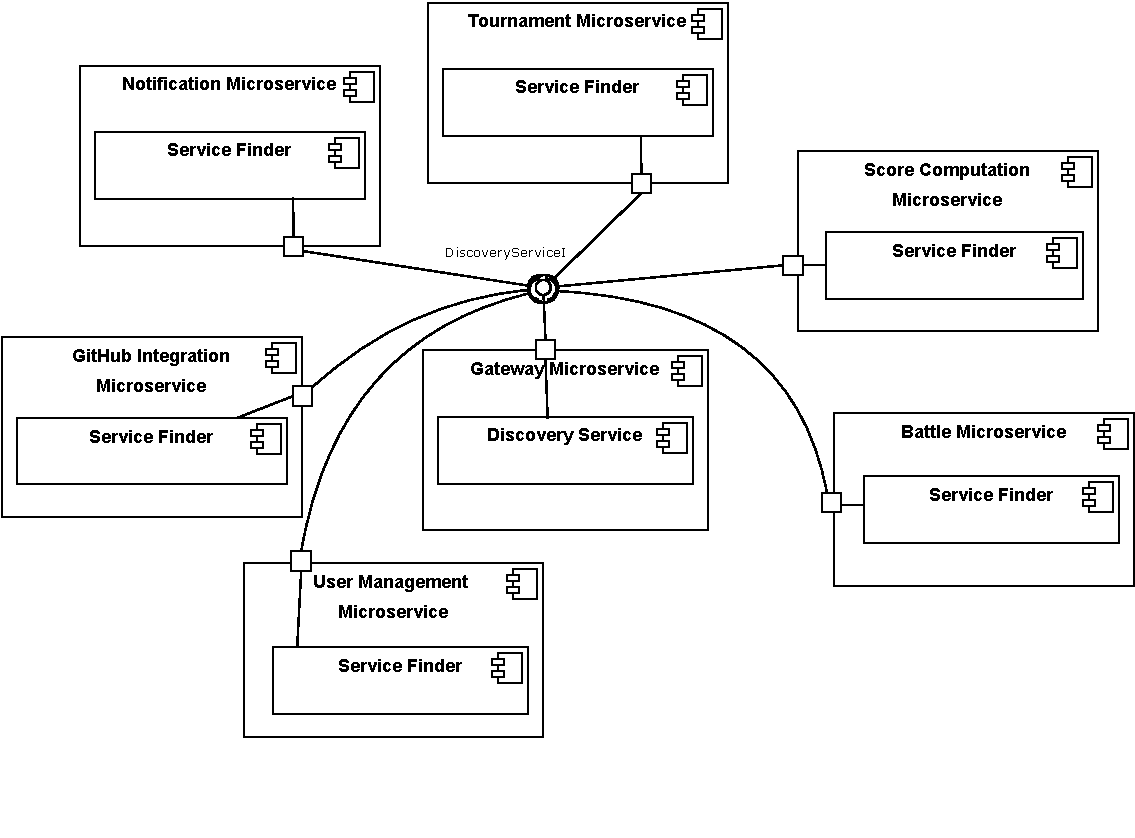
\includegraphics[width=\linewidth]{2Component_ServiceDiscovery}
	
\end{minipage}

	The interpretation is quite simple. The Gateway Microservice contains a component called Discovery Service, which is the software component that implements the logic to offer the discovery service. The Discovery Service component exposes an API (DiscoveryServiceI), that can be used by all other microservices in order to locate each other. 

\subsubsection{Event-driven pattern components}
\begin{minipage}{\linewidth}
	This section illustrates all the components that are needed in the system in order to implement an asynchronous, event-driven communication between microservices. This design choice has been taken in order to lighten up the system in specific interactions between microservices that would otherwise require a computationally expensive synchronous communication.
	
	The following diagram shows the major components that help achieve an event-driven architecture:
	
	\vspace{2cm}
	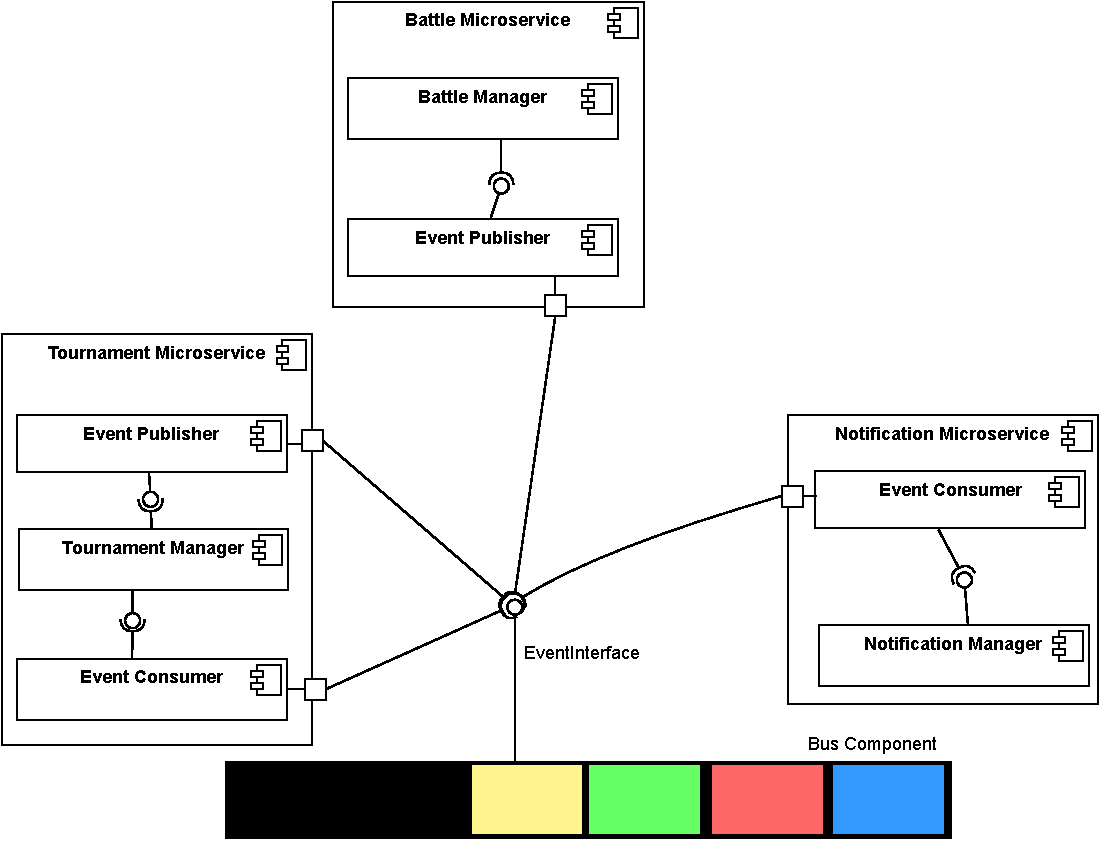
\includegraphics[width=\linewidth]{3Component_EventDriven}
	
	\vspace{2cm}
	
\end{minipage}

The most important element is the Bus component, which can be thought of as a queue of messages or events. Microservices in the \app system can either produce events (i.e. push events on the queue) or consume events (i.e. read events on the queue) and take actions accordingly.

It is important to mention that this representation is purposely general and not tied up with any specific software product, framework or implementation. The concrete way in which this design is achieved is left to the implementation of the product.

From the diagram, it is possible to see that only some microservices are illustrated, which are the only one exploiting this mechanism to communicate and interact. 
Inside these microservices, there is an Event Publisher component if the microservice has to be able to publish events on the Bus, and there might be an Event Consumer component in case the microservice has to be able to read from the Bus the events that are queued.

The Tournament Microservice, for instance, has both the Event Publisher component and the Event Consumer component. Indeed, the Tournament Microservice has to publish an event every time a new tournament is created or closed. At the same time, the tournament has to be able to read from the bus when a battle is finished, to take actions accordingly. 

The Battle microservice only publishes events when the battle is created and terminates.

The Notification Microservice is the one always listening to upcoming events in order to fabricate the correct notifications for the users of the \app platform.




\subsubsection{Data layer access component diagram}
\begin{minipage}{\linewidth}
	This diagram proposes a convenient view to see how the access is performed by the various microservices on the shared data layer (shared DBMS).
	
	\vspace{2cm}
	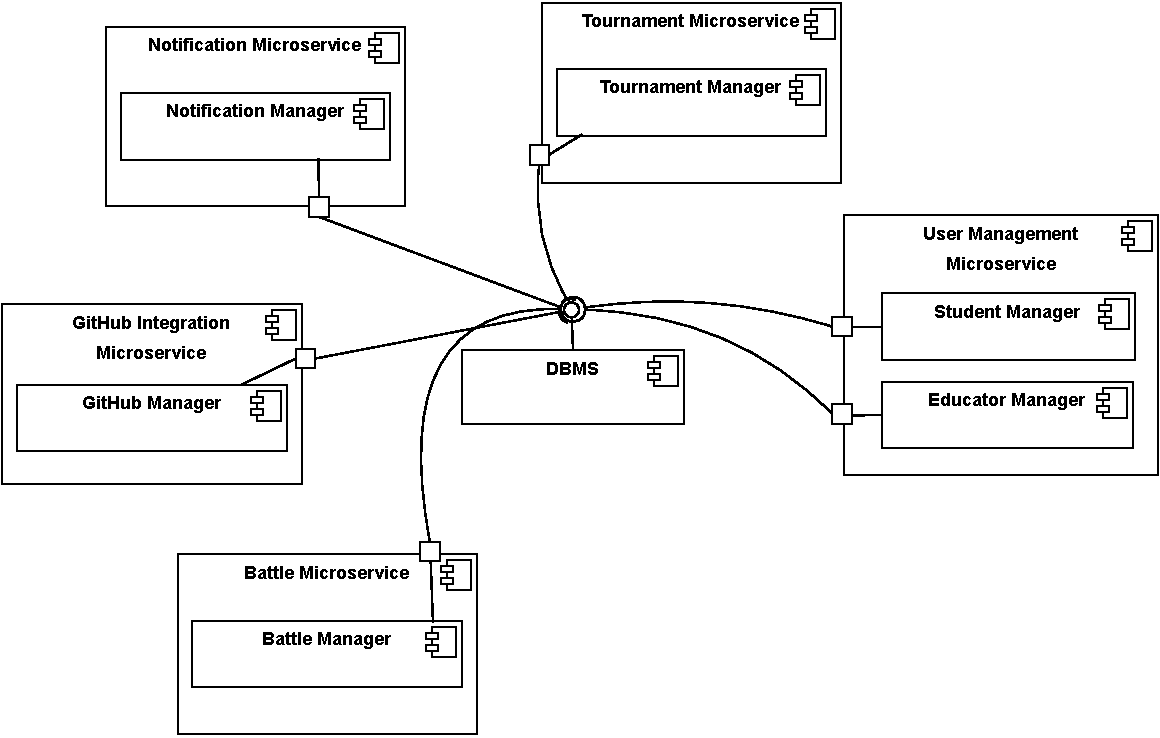
\includegraphics[width=\linewidth]{4Component_DataAccess}
	
	\vspace{2cm}
	
	The DBMS exposes an interface that is employed by all microservices to work with the persistent data stored in the DBMS.
	
	Looking at every microservice individually, it is possible to notice that they all are equipped with a "Manager" component, which is responsible for manipulating and accessing data.
	
	Every microservice of the \app application is responsible for a different section of the data domain. For instance, the Tournament microservice only works on the data stored in the shared DBMS that is related to tournaments and offers to the other microservices all the relevant information about tournaments that might be needed.
	

\end{minipage}

\subsubsection{User interfaces component diagram}
\begin{minipage}{\linewidth}
	This diagram proposes a convenient view of the system for what concerns user interfaces. The design choices that have been taken in the \app system as concerns the user interfaces can be summed up in this way:
	
	\begin{itemize}
		\item The different interfaces that are offered to the user are not gathered in a single component, but they are scattered across the various microservices. This decision is due to the fact that different UIs offer different views on the data of the application. Therefore, some microservices (working on a specific section of the data domain) might be more suitable for providing a specific user interface than others.
		\item All the times a user interface is offered to the user, the Gateway Microservice handles the transmission of data, standing in between the user and the access to the internal microservice. Therefore, all the UIs content passes by the Gateway before reaching the client user.
	\end{itemize}
	
	This diagram tries to illustrate the two points of the above list, by representing a View component inside each microservice that is responsible for building and offering specific user interfaces when required. 
	The Gateway microservice intercepts the user's requests and when a new UI is needed, it contacts the correct microservice that will supply it.
	
	
	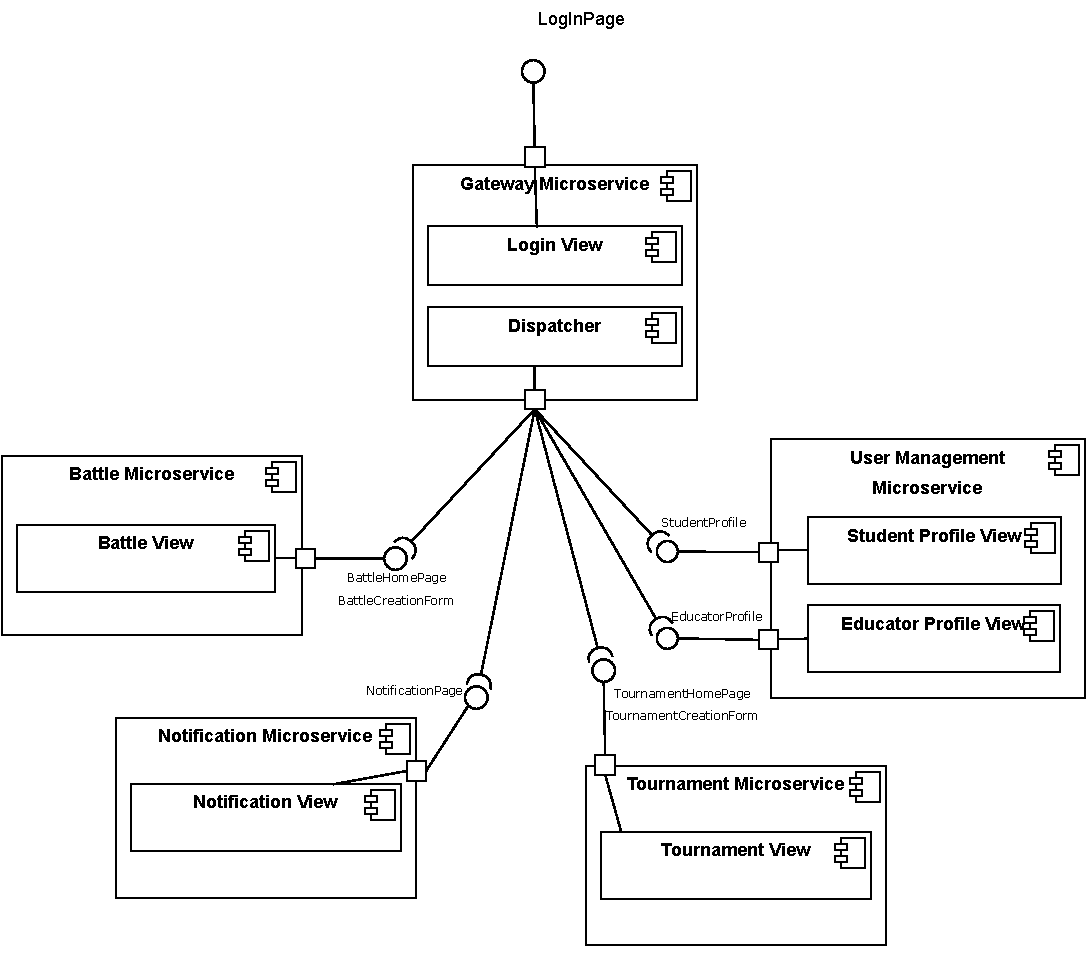
\includegraphics[width=\linewidth]{5Component_ViewsUI}
	
	
	
\end{minipage}
\subsection{Deployment View}
The deployment view addresses the how and where of the \app system's execution, examining the distribution of components, the orchestration of services, and the overall infrastructure that supports the software. In other terms, this section is dedicated to a mapping between software artifacts that implement the logic that makes \app work and the hardware devices that are needed to concretely execute them.

This document aims to provide a comprehensive understanding of the architectural choices that facilitate efficient resource utilization, scalability to meet varying workloads, and the ability to adapt to evolving operational requirements. 

As in the previous sections, this view of the system is provided through multiple diagrams that go deeper and deeper into the details of the deployment environment. These diagrams are not exclusive to one another, rather they should be seen as a hierarchical illustration of the same concept, from a more high-level approach, to a more detailed insight.



\subsubsection{High-level Deployment View}
\begin{minipage}{\linewidth}
This diagram shows the bare minimum set of components that are needed to illustrate the deployment view for the \app system.

\vspace{1cm}
\begin{center}
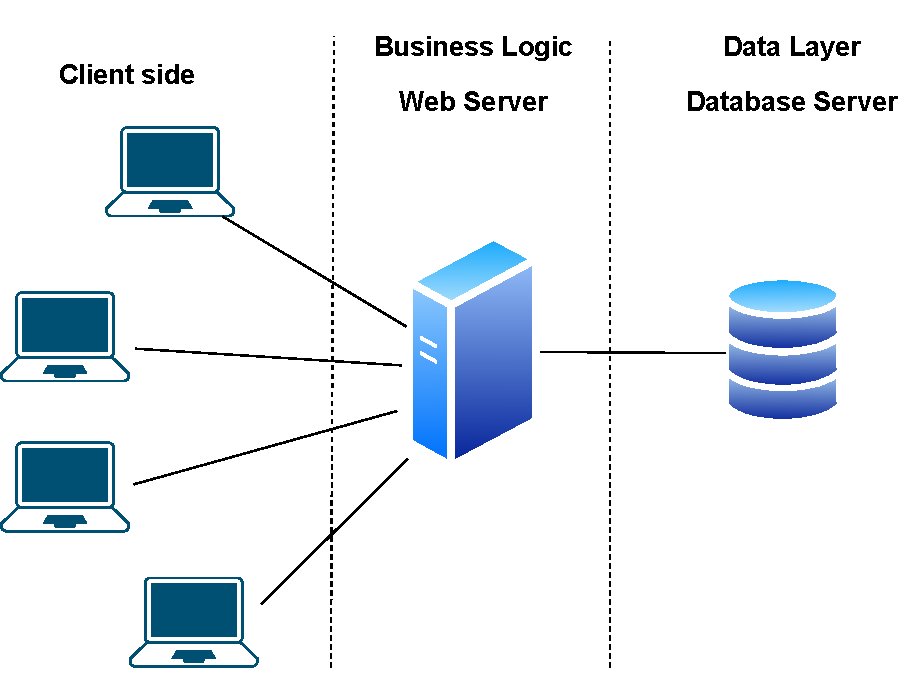
\includegraphics[width=0.7\linewidth]{1Deployment_High_Level}
\end{center}
\vspace{1.5cm}

\end{minipage}

As it is possible to see from the figure, from a deployment perspective, the \app platform can be classified as a three-tier architecture. The three distinct areas in the illustration represent the three tiers (layers) of the architecture, more specifically the client users (on the left), the server (in the center) and the data layer (on the right).

All users are equipped with a device with internet connection that is able to send and receive requests to the server hosting \app. The entire \app is hosted on a single remote server, where all microservices are launched as separate programs, interacting with each other. The data layer can be implemented with a remote Database server that provides persistent data support to the whole system.

This deployment architecture is very convenient for a series of reasons. First off, it allows for a complete separation of concerns between the various layers, in particular between the business logic of the application (hosted on the server) and the data layer (in the DBMS). Moreover, it is an extensible architecture that can be further developed and enlarged in order to accommodate for a varying workload. For instance, the data layer can be replicated on multiple servers, in order to increase performance for accessing and manipulating data. This same strategy can be adopted for the business layer in case of necessity.

\subsubsection{Detailed Deployment View}

\begin{minipage}{\linewidth}
	The following representation offers some more insights on how the software artifacts that implement the various components of the \app application map onto hardware elements.
	
	\vspace{2cm}
	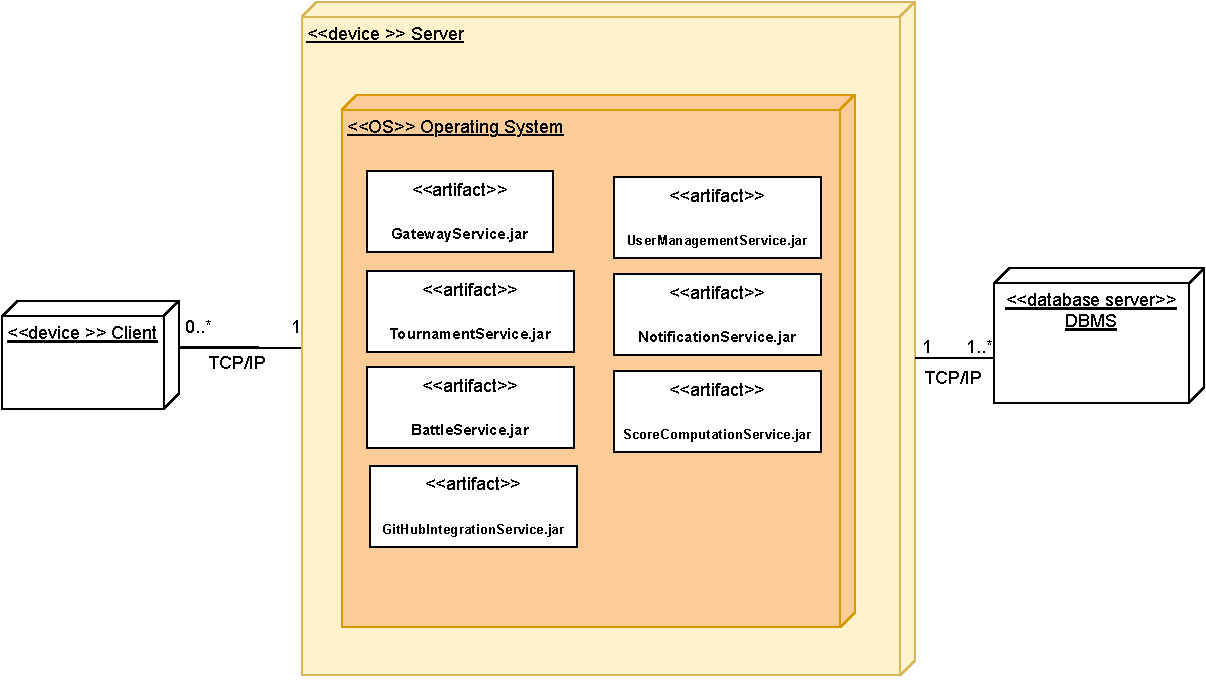
\includegraphics[width=\linewidth]{2DeploymentArtifacts}
	\vspace{1.5cm}
	
\end{minipage}

The major elements in the representation are still the same as in the previous description. On the left, the client side, equipped with a device that has internet access in order to communicate with the server over a TCP/IP protocol. The multiplicity specifications on the line that connects the client with the server shows that many clients can be interacting with the server simultaneously.

The server is the big box at the center of this diagram. The UML deployment diagram offers the possibility to show the execution environment of the \app system by nesting multiple boxes. 

All the microservices artifacts are mapped onto the single server instance. Indeed they are executed as separate processes inside the server machine.

Finally, on the right hand side, there is the data layer, which consists of a database server that is connected to the central server over the internet as well (TCP/IP protocol). 

This design has been chosen because it allows for smooth and easy extension of the system whenever it is needed. 
For instance, the DBMS can be replicated multiple times, in order to parallelise the requests coming from the server. 
If a more advanced distributed architecture was needed, the artifacts implementing the various microservices could simply be split across different nodes of the network and the overall system would still work correctly (with some settings and configurations).
The microservices themselves could be replicated inside the server machine in order to boost performance even more.
 


\subsection{Run Time View}

This section provides a detailed perspective on how the system internally works and its component interact with each other at runtime. It focuses on the dynamic aspects of the software, emphasizing the flow of control, data, and communication between different modules or components.\newline
Just as a note, in order to make the diagrams more readable, some abbreviations have been used in the methods exposed by the various interfaces of \app components (as shown in section 2.5). In particular, tournamentName is tName, battleName is bName.


\subsubsection*{Educator login}
\begin{figure}[h!]
    \centering
    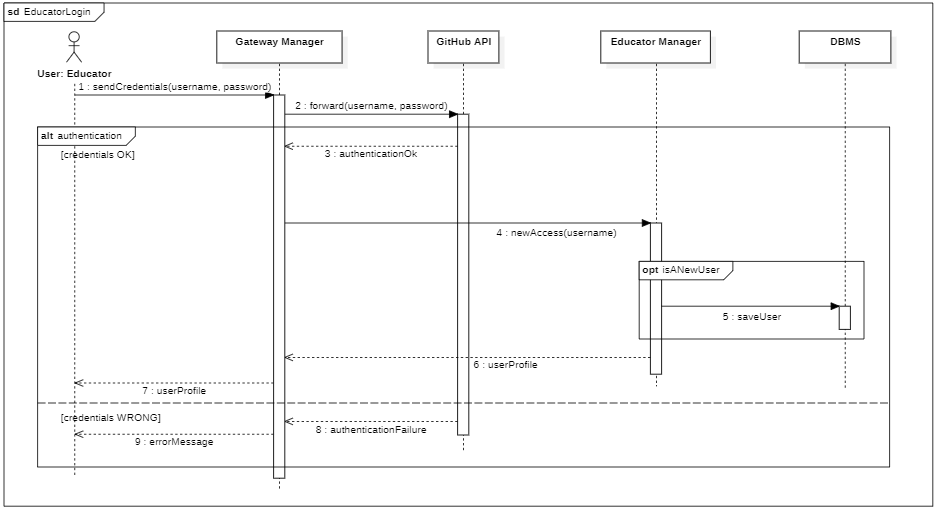
\includegraphics[width=1\linewidth]{1Sequence_EducatorLogIn}
    \caption{Runtime view of the login of an educator}
    \label{fig:educator_login}
\end{figure}

The educator login process unfolds in the following manner: the Educator initiates the login by contacting the Gateway Manager and transmitting their credentials. Subsequently, the Gateway Manager interfaces with the GitHub API to verify and authorize access. Two possible scenarios may unfold: a successful authentication or an unsuccessful one. In the latter case, an error message is generated and displayed to the Educator. In the event of a successful authentication, the Gateway Manager communicates with the Educator Manager, forwarding all relevant data to be stored in case it is the Educator's first sign-in. In both scenarios, the Educator Manager is responsible for returning the user profile to the Educator.

This process ensures a seamless and secure login experience, with appropriate feedback provided to the Educator based on the outcome of the authentication process.
\newpage

\subsubsection*{Student login}
\begin{figure}[h!]
    \centering
    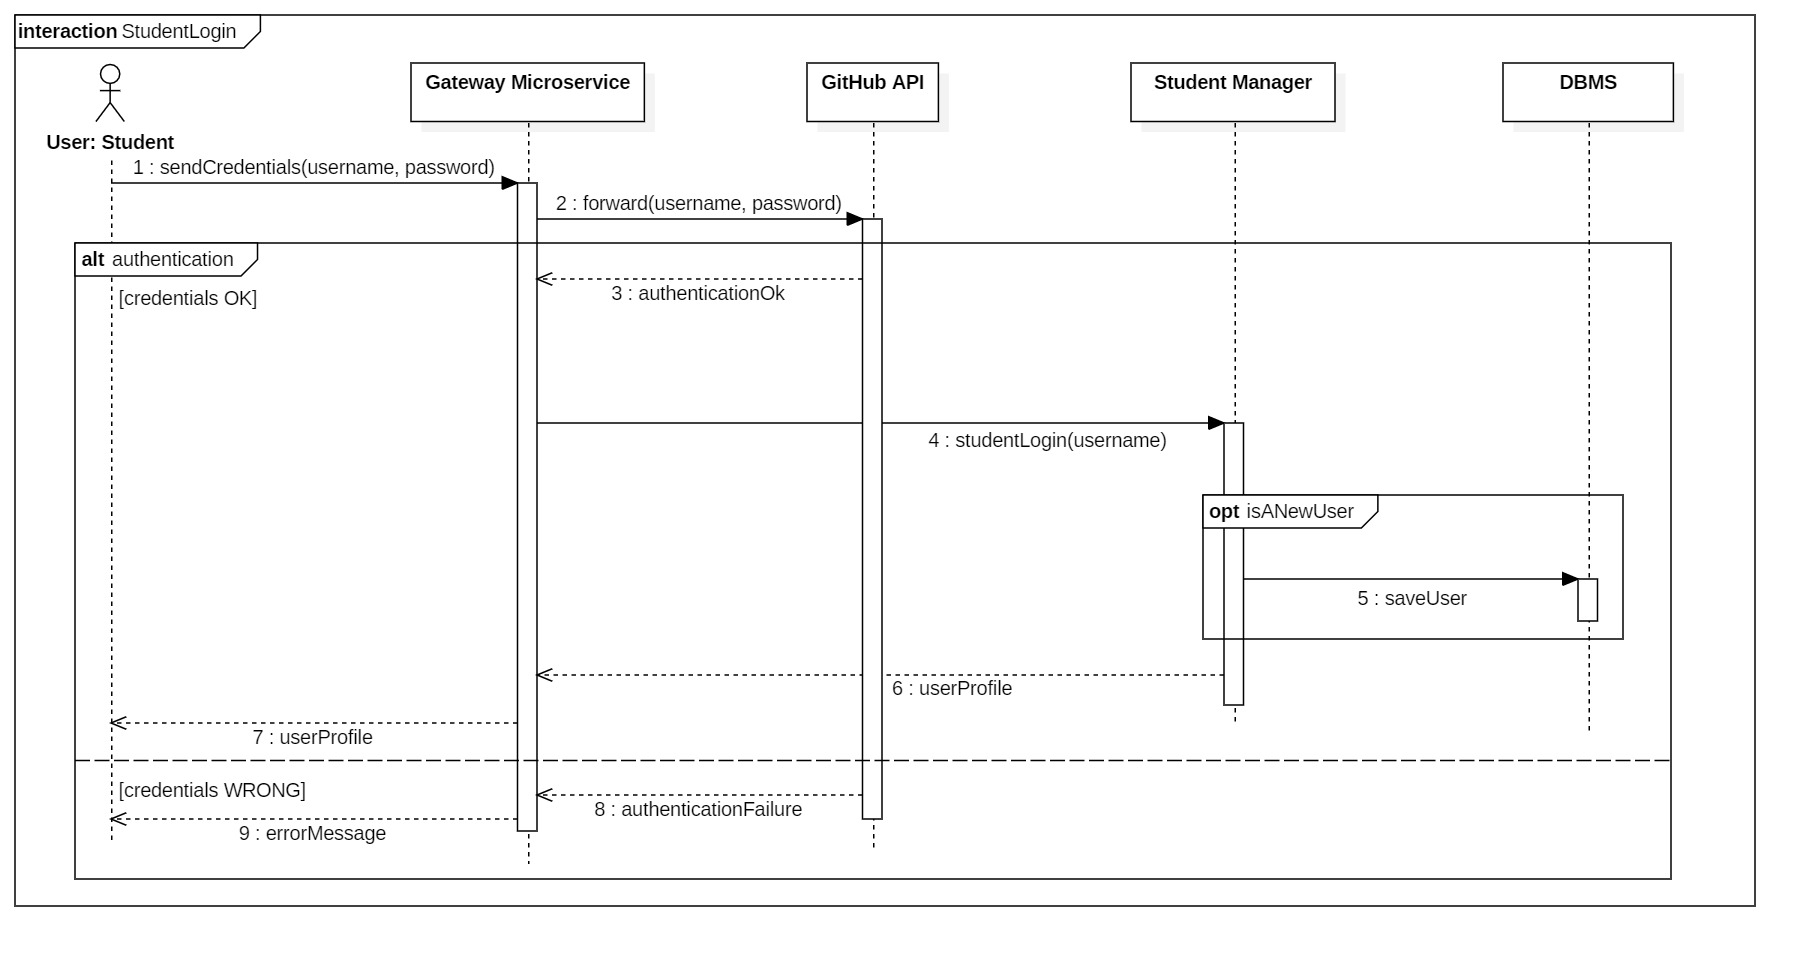
\includegraphics[width=1\linewidth]{2.ArchitecturalDesign/res/StudentLogin.jpg}
    \caption{Runtime view of the login of a student}
    \label{fig:student_login}
\end{figure}

The student login process mirrors that of the educator, with the primary distinction lying in the actor, now the student, and the involvement of different microservices. Here's how it unfolds: the Student initiates the login process by reaching out to the Gateway Manager and submitting their credentials. Subsequently, the Gateway Manager interfaces with the GitHub API to validate and authorize access.

Similar to the educator's login process, two potential outcomes are possible: a successful authentication or an unsuccessful one. In the case of an unsuccessful authentication, an error message is generated and presented to the student. However, in the event of a successful authentication, the Gateway Manager now communicates directly with the Student Manager. The Student Manager is then responsible for handling the data, including storage in the case of the student's initial sign-in, and returning the user profile to the student.

Despite the differences in actors and microservices, the student login process ensures a comparable and secure user experience, tailored to the specific needs of the student user role.

\newpage

\subsubsection*{Tournament creation}
\begin{figure}[h!]
    \centering
    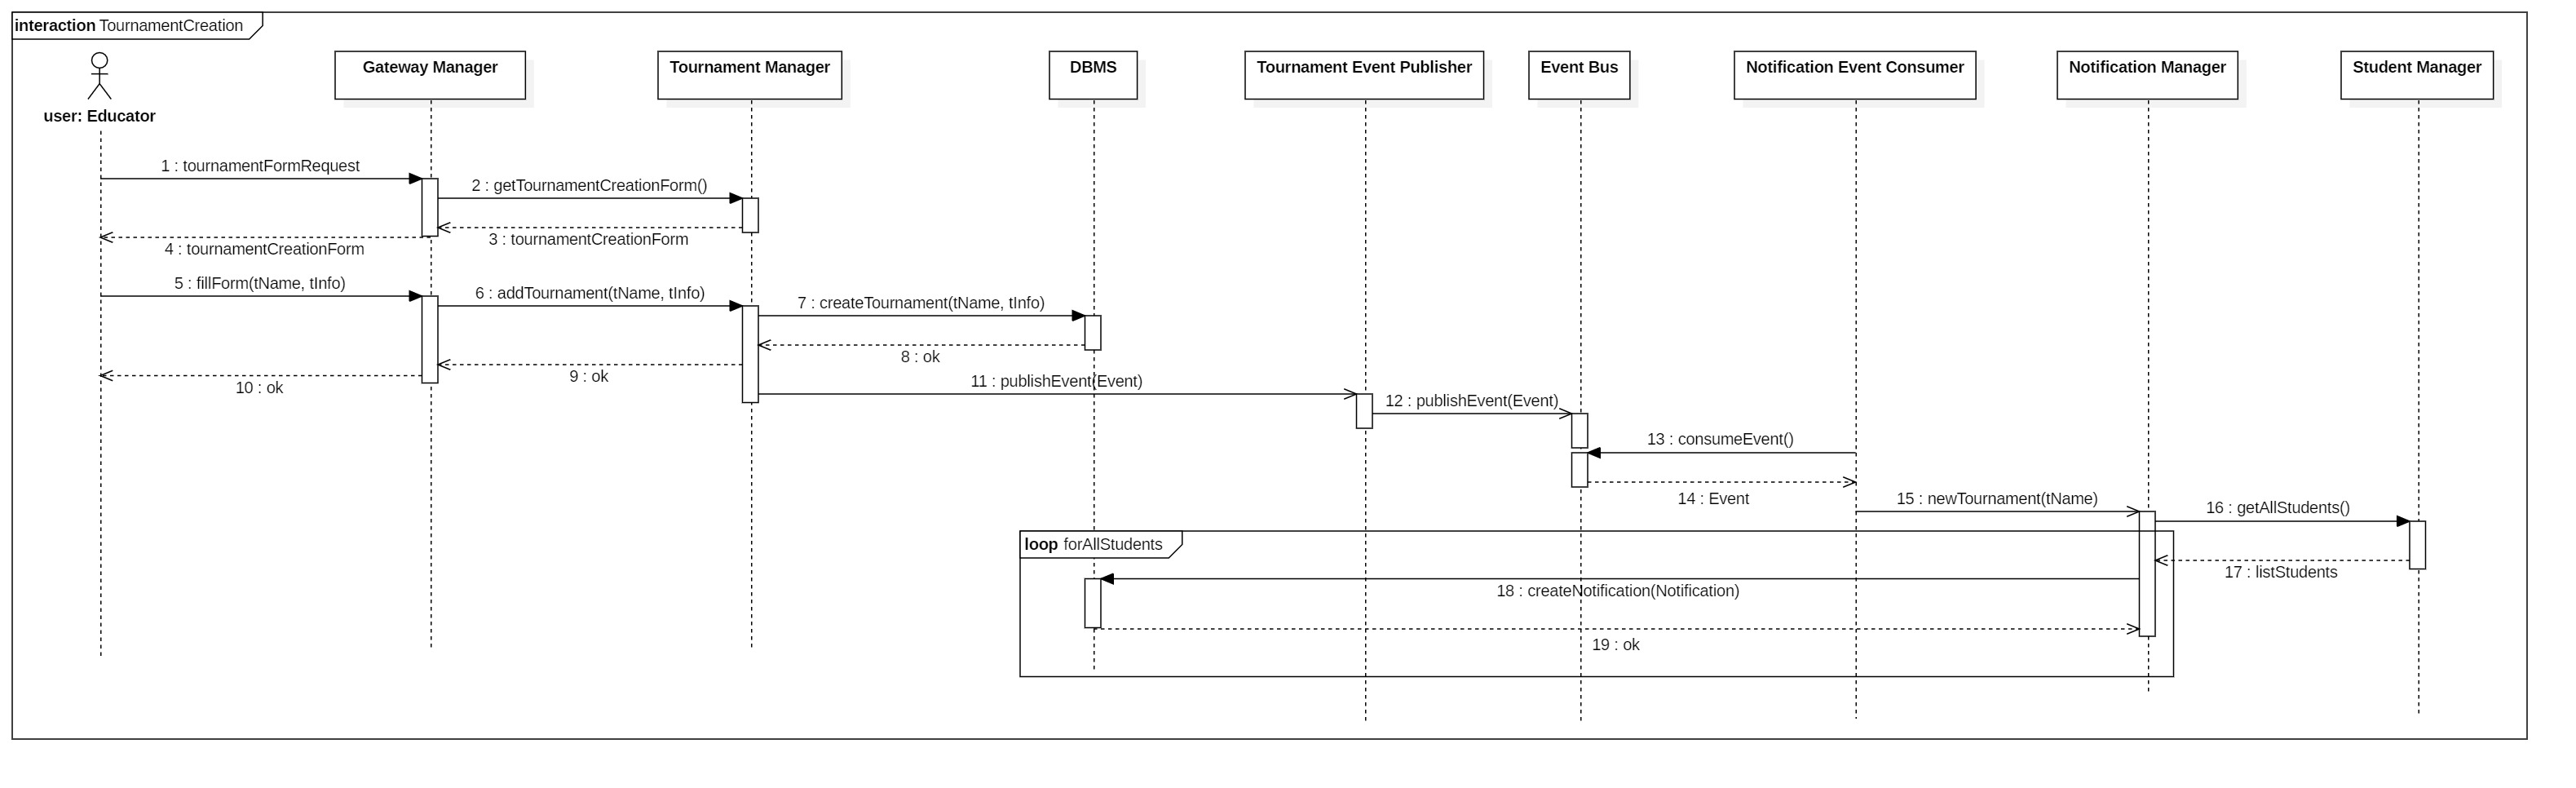
\includegraphics[width=1.3\linewidth, angle=90]{2.ArchitecturalDesign/res/TournamentCreation.jpg}
    \caption{Runtime view of the creation of a tournament}
    \label{fig:tournament_creation}
\end{figure}

In Figure \ref{fig:tournament_creation}, the diagram illustrates the interactions between components when an educator initiates the creation of a new tournament. Initially, the educator contacts the Gateway Manager, which then sends a request to the Tournament Manager in order to obtain the form necessary for the creation process. After receiving the form, the educator fills it out and sends it back to the Tournament Manager. The Tournament Manager stores the information in the DBMS and triggers a notification to signify the successful creation of the tournament. 

While the specific details of this notification process will be discussed momentarily, it is worth noting that this sequence remains consistent across various runtime views and will be omitted in subsequent descriptions.

Subsequently, the Tournament Publisher receives the data pertaining to the newly created tournament and communicates with the Event Bus to publish this information. Then, asynchronously, the Notification Consumer polls the Event Bus, retrieving the new event. Once obtained, the Notification Consumer generates a notification and forwards it to the Student Manager. The Student Manager then iterates through all the students, ensuring each receives the notification.

\newpage

\subsubsection*{Battle creation}
\begin{figure}[h!]
    \centering
    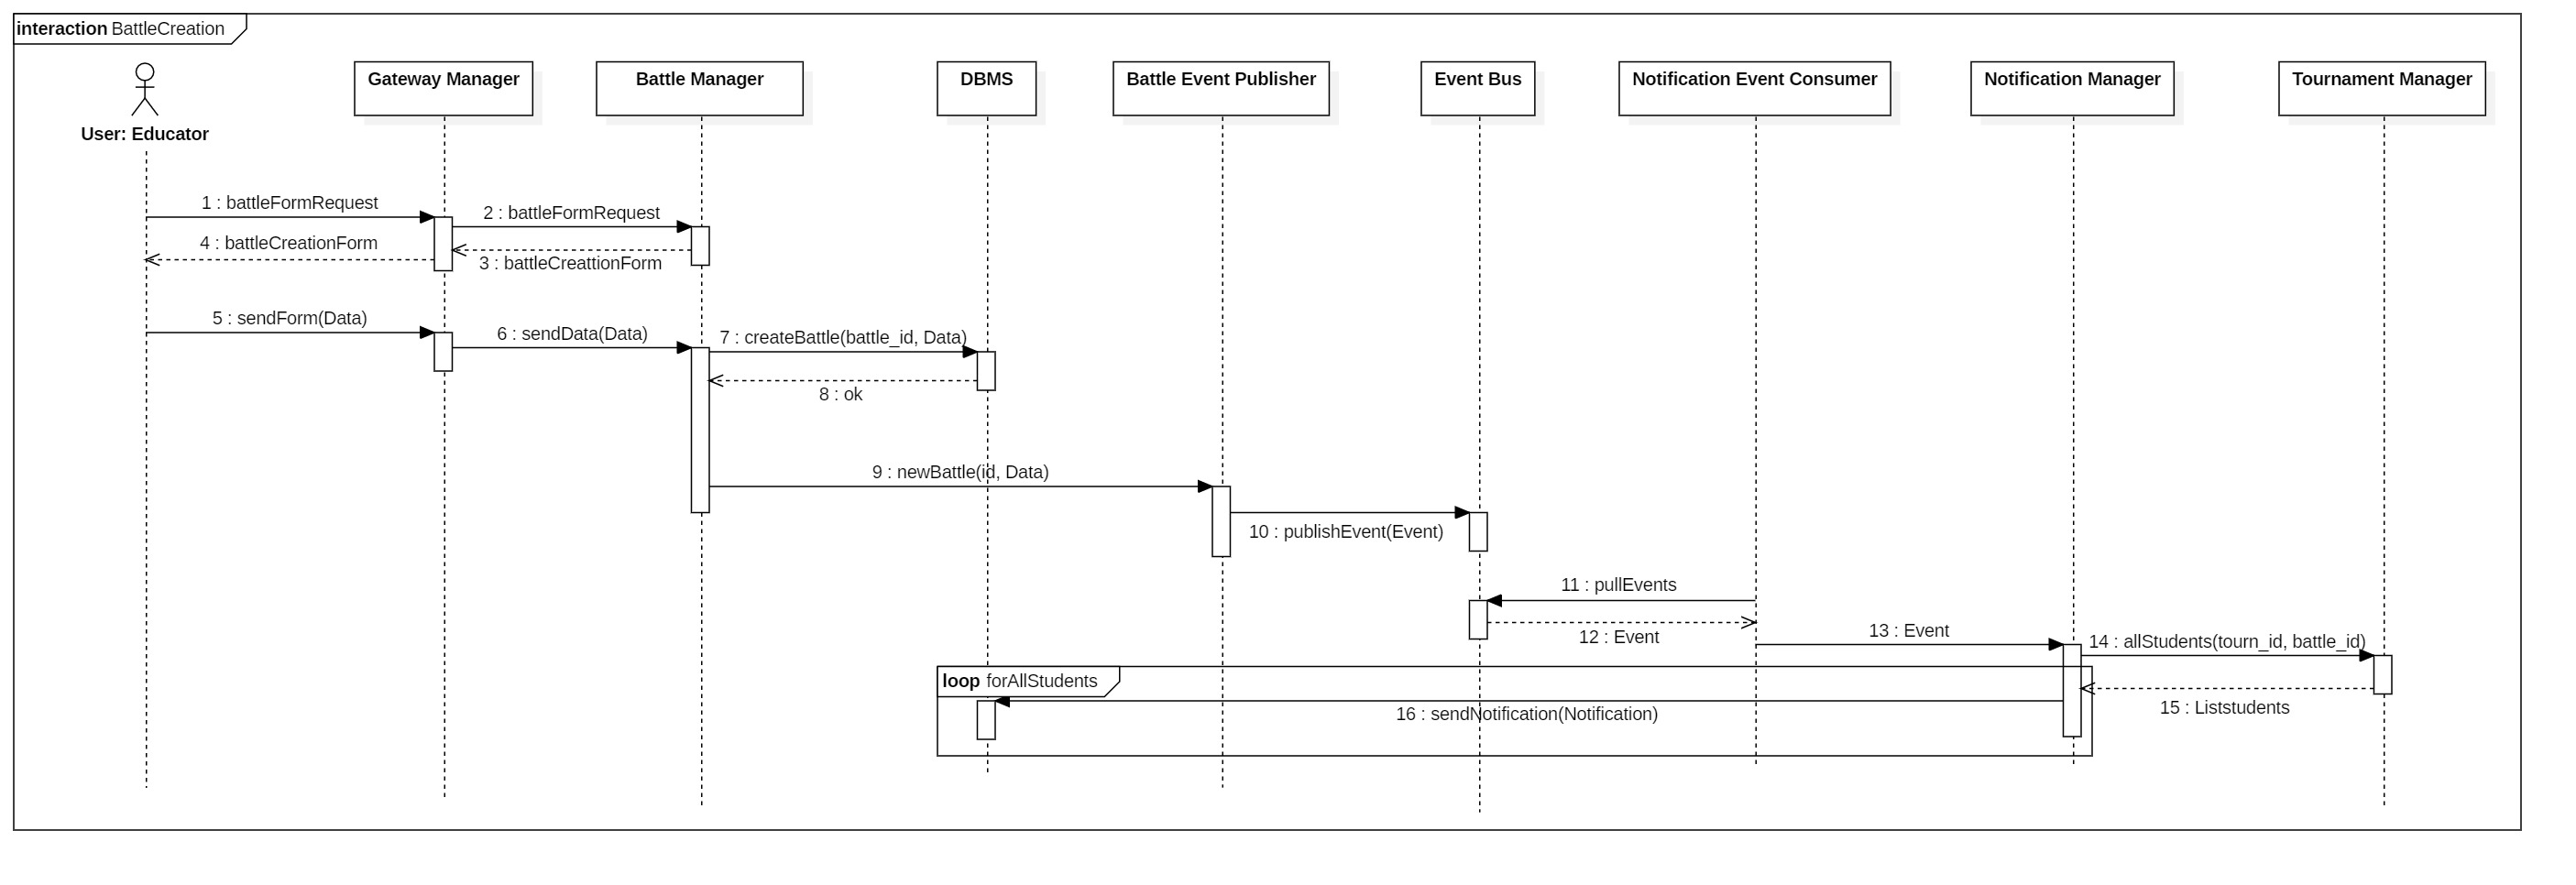
\includegraphics[width=1.3\linewidth, angle=90]{2.ArchitecturalDesign/res/BattleCreation.jpg}
    \caption{Runtime view of the creation of a battle}
    \label{fig:battle_creation}
\end{figure}

The process for battle creation mirrors that of tournaments. The Educator initiates the process by sending a request to the Gateway Manager, which forwards the request to the Battle Manager. The Battle Manager responds by providing the necessary form for the Educator to complete. Subsequently, the Educator fills out the form and returns it to the Battle Manager. The Battle Manager then stores the information for the newly created battle in the DBMS. Similar to the tournament creation, a new event is generated.

It's important to note that, in this context, all the students notified will only be those subscribed to the tournament in which the battle has been created.

\newpage

\subsubsection*{End of a tournament}
\begin{figure}[h!]
    \centering
    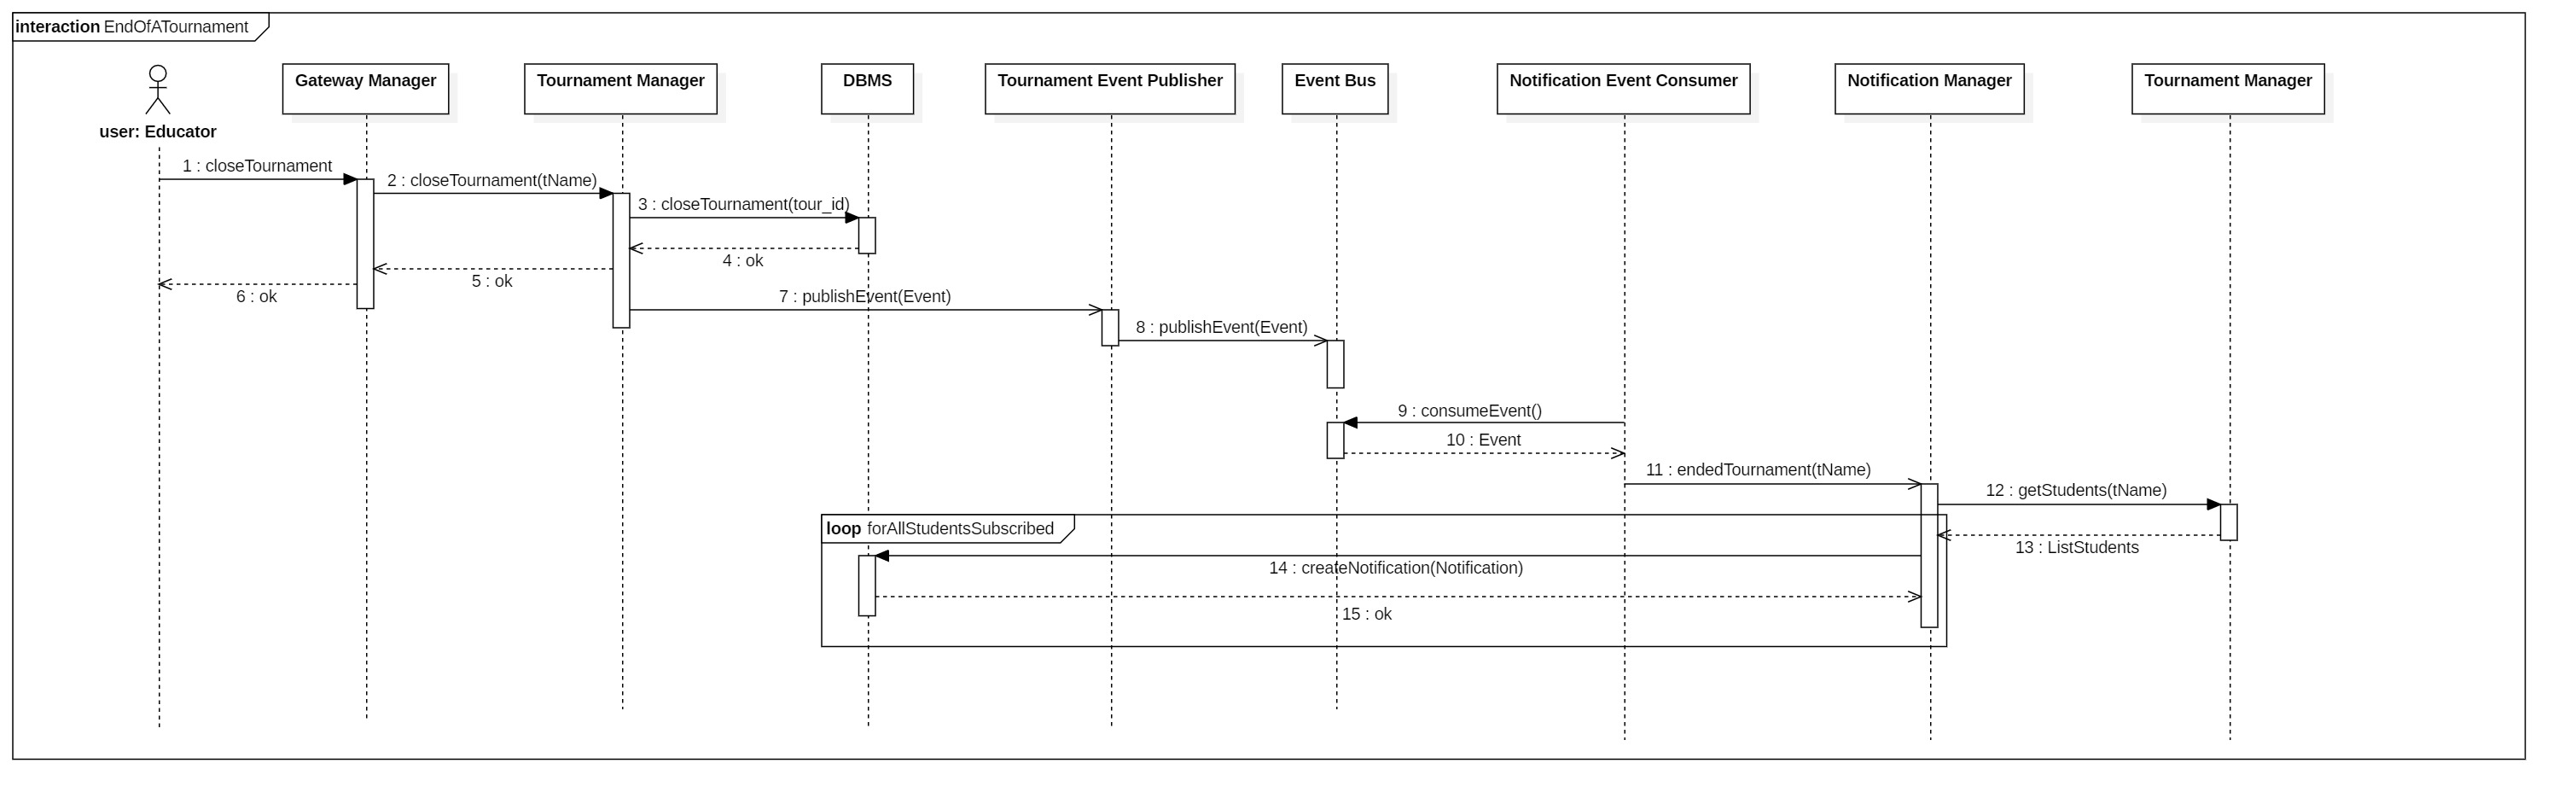
\includegraphics[width=1.3\linewidth, angle=90]{2.ArchitecturalDesign/res/EndOfATournament.jpg}
    \caption{Runtime view when the end of a tournament is reached}
    \label{fig:tournament_end}
\end{figure}

When a tournament concludes, the determination is made by the Educator, who initiates the process by sending a request to the Gateway Manager. The Gateway Manager then forwards this request to the Tournament Manager, which in turn updates the relevant data regarding the tournament in the DBMS. Following the update, a new event is generated and disseminated to all the students who have subscribed to that particular tournament, adhering to the previously outlined notification mechanism.

\newpage

\subsubsection*{End of a battle}
\begin{figure}[h!]
    \centering
    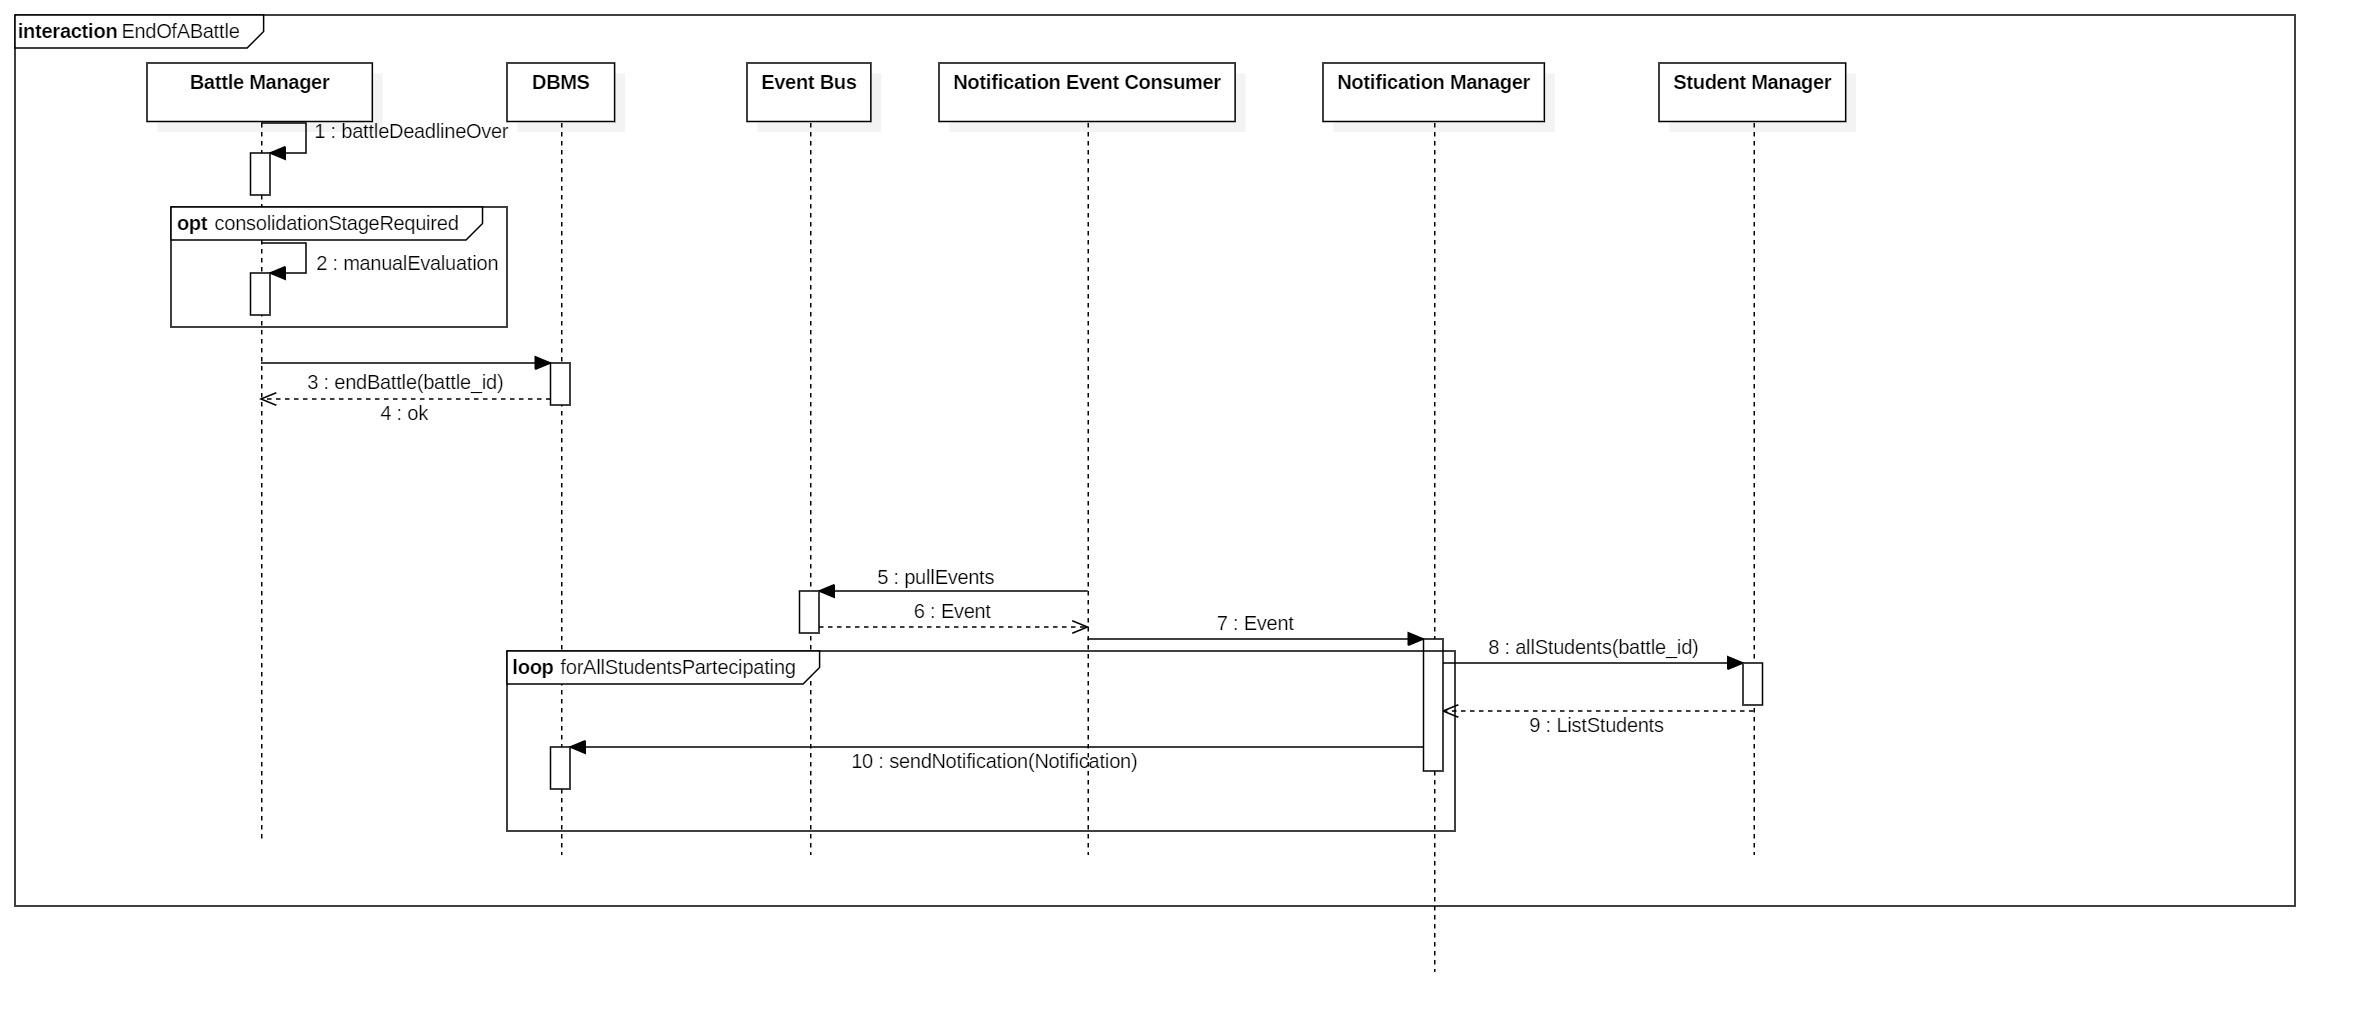
\includegraphics[width=1.3\linewidth, angle=90]{2.ArchitecturalDesign/res/EndOfABattle.jpg}
    \caption{Runtime view when a battle ends}
    \label{fig:battle_end}
\end{figure}

The conclusion of a battle occurs upon reaching its specified deadline, and the mechanism for monitoring this may involve a polling system, depending on the chosen development framework. Once the deadline is reached, the system checks whether a manual evaluation is required, as determined during the battle's creation. Subsequently, the parameters of the battle are updated by interacting with the DBMS. Following this update, an event is generated, mirroring the previously described process, and disseminated accordingly.

\newpage

\subsubsection*{Subscribe To Tournament}
\begin{figure}[h!]
    \centering
    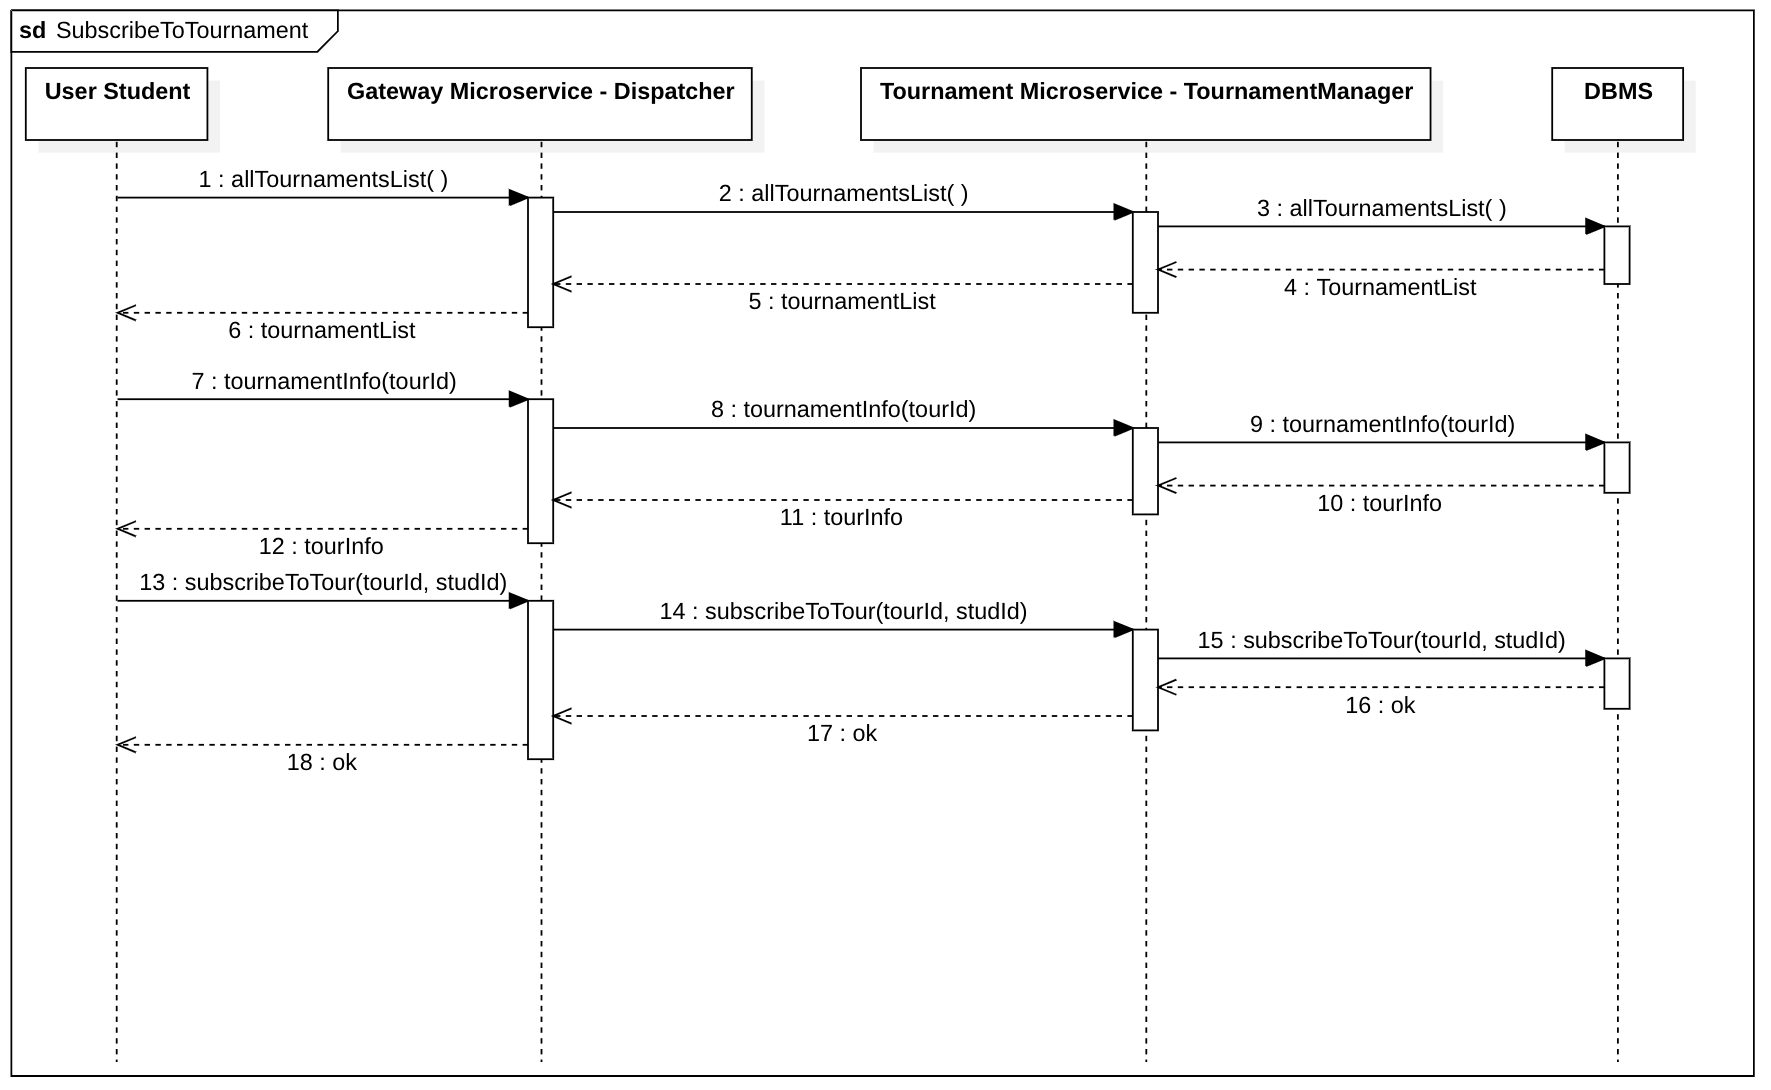
\includegraphics[width=1\linewidth]{2.ArchitecturalDesign/res/subscribeToTournament.jpg}
    \caption{Runtime view when a student subscribes to a tournament}
    \label{fig:subsTournament}
\end{figure}

The client initiates a request for a list of tournaments. This request is transmitted to the gateway component, which acts as an intermediary.
The gateway, upon receiving the request, forwards it to the Tournament Manager microservice. The Tournament Manager retrieves the relevant information from the database and subsequently transmits the data back to the gateway.
The gateway, in turn, relays the tournament list to the client.\\
Subsequently, the client initiates a request for specific information about a particular tournament. This request traverses the gateway before reaching the Tournament Manager microservice. The Tournament Manager retrieves the requisite details from the Database Management System (DBMS) and transmits the information back.\\
Lastly, the client issues a subscription request. This request is routed through the gateway to the Tournament Manager. The Tournament Manager processes the request by writing the new subscription details to the DBMS, thereby completing the subscription process. After the processs is completed a confirmation message is trasmitted back.

\newpage

\subsubsection*{Subscribe To Battle}
\begin{figure}[h!]
    \centering
    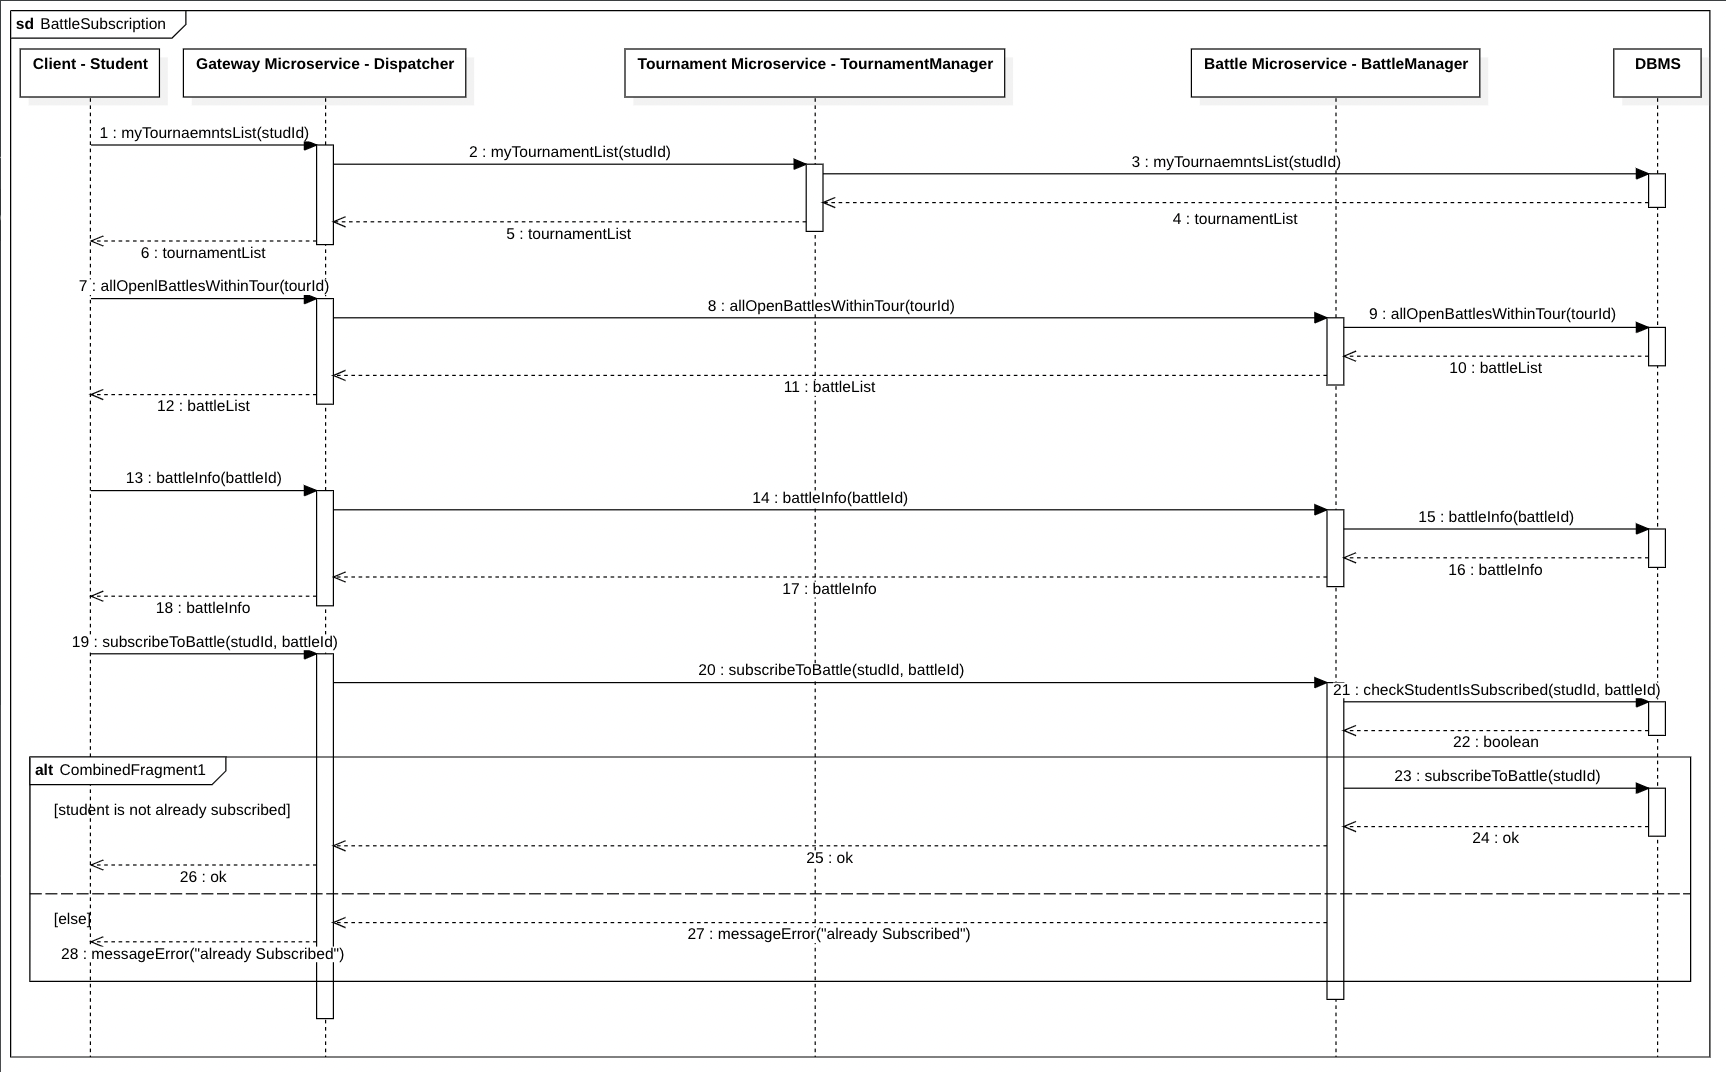
\includegraphics[width=1.3\linewidth, angle=90]{2.ArchitecturalDesign/res/subscribeToBattle.png}
    \caption{Runtime view when a student subscribes to a battle}
    \label{fig:subsBattle}
\end{figure}

The sequence begins with the client initiating a request for the list of tournaments. This request is directed to the gateway component.
The gateway, acting as an intermediary, forwards the tournament list request to the Tournament Manager microservice. The Tournament Manager retrieves the pertinent information from the Database Management System (DBMS) and transmits it back to the gateway.
Subsequently, the gateway relays the tournament list to the client.\\
Following this, the client makes a request for the list of battles within a specific tournament, specifically those currently open for subscription. This request is initially routed through the gateway before being further directed to the Battle Manager microservice.
The Battle Manager, upon receiving the request, retrieves the relevant information from the database and sends the list of open battles back through the gateway to the client.\\
Subsequently, the client sends a subscription request for a specific battle. The subscription request first traverses the gateway and then reaches the Battle Microservice.
Within the Battle Microservice, the system checks the database to verify if the student is already subscribed to the specified battle. If the student is already subscribed, an error message is generated and transmitted back to the client.
If the student is not already subscribed, the Battle Manager writes the new subscription details to the database and generates a confirmation of the subscription.
The confirmation of the subscription is then sent back through the gateway to the client.

\newpage

\subsubsection*{Educator Gives Permission}
\begin{figure}[h!]
    \centering
    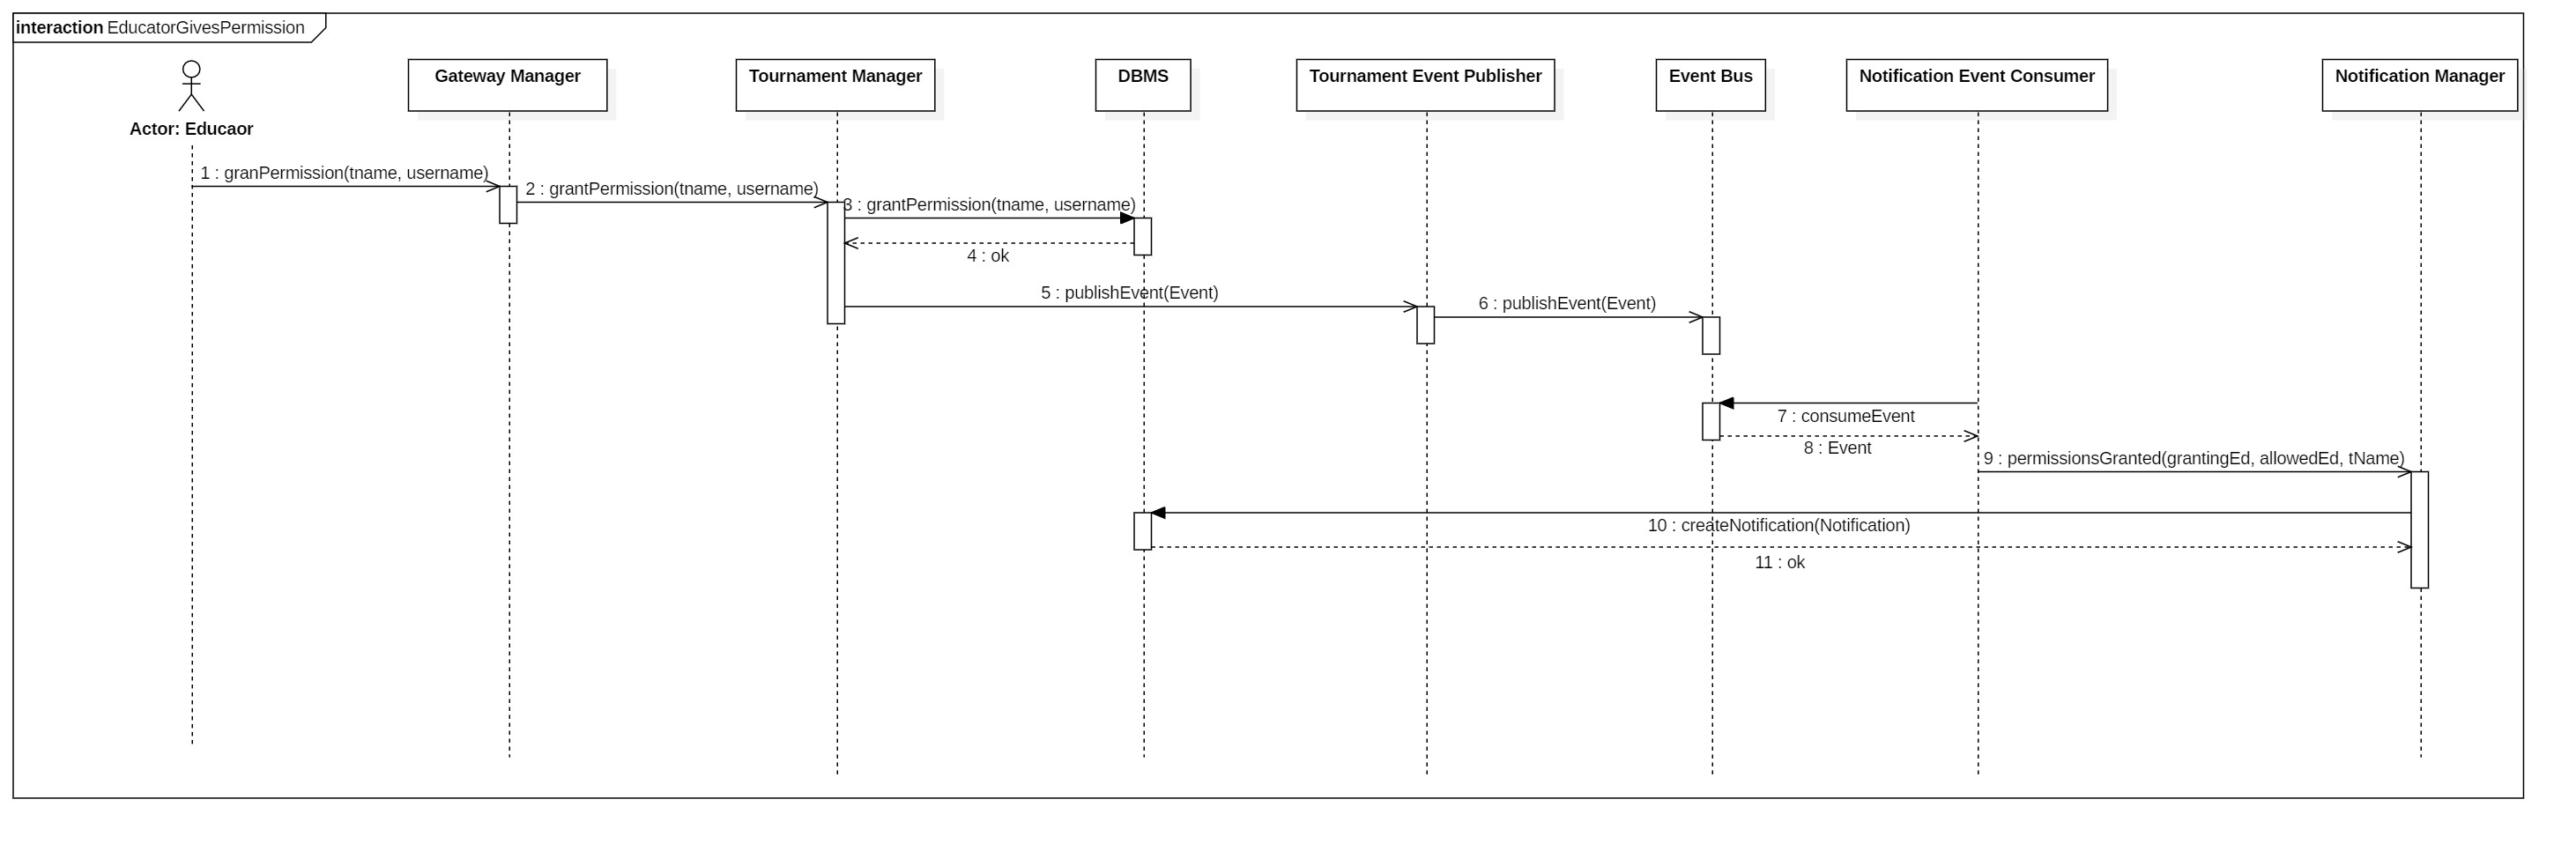
\includegraphics[width=1.3\linewidth, angle=90]{2.ArchitecturalDesign/res/EducatorGivesPermission.jpg}
    \caption{Runtime view of the educator giving permission to another one for a tournament he owns}
    \label{fig:permission}
\end{figure}

The sequence starts with the Educator engaging with the Gateway Manager to request the possibility of grant permission for a tournament they own. To do this, the Educator sends a request that includes the tournament name and their username for identification.
The Gateway Manager then redirects the request to the appropriate component, the Tournament Manager, which saves the new information in the Database by interacting with the DBMS, receiving then an affirmative response.
After completing this step, the Tournament Manager must generate a new Notification. As mentioned earlier, the Publisher publishes the new Event to the Event Bus, and the Notification Event Consumer, in collaboration with the Notification Manager, creates the new Notification, saving it into the Database with the assistance of the DBMS component.

\newpage

\subsubsection*{Badge Assignment}
\begin{figure}[h!]
    \centering
    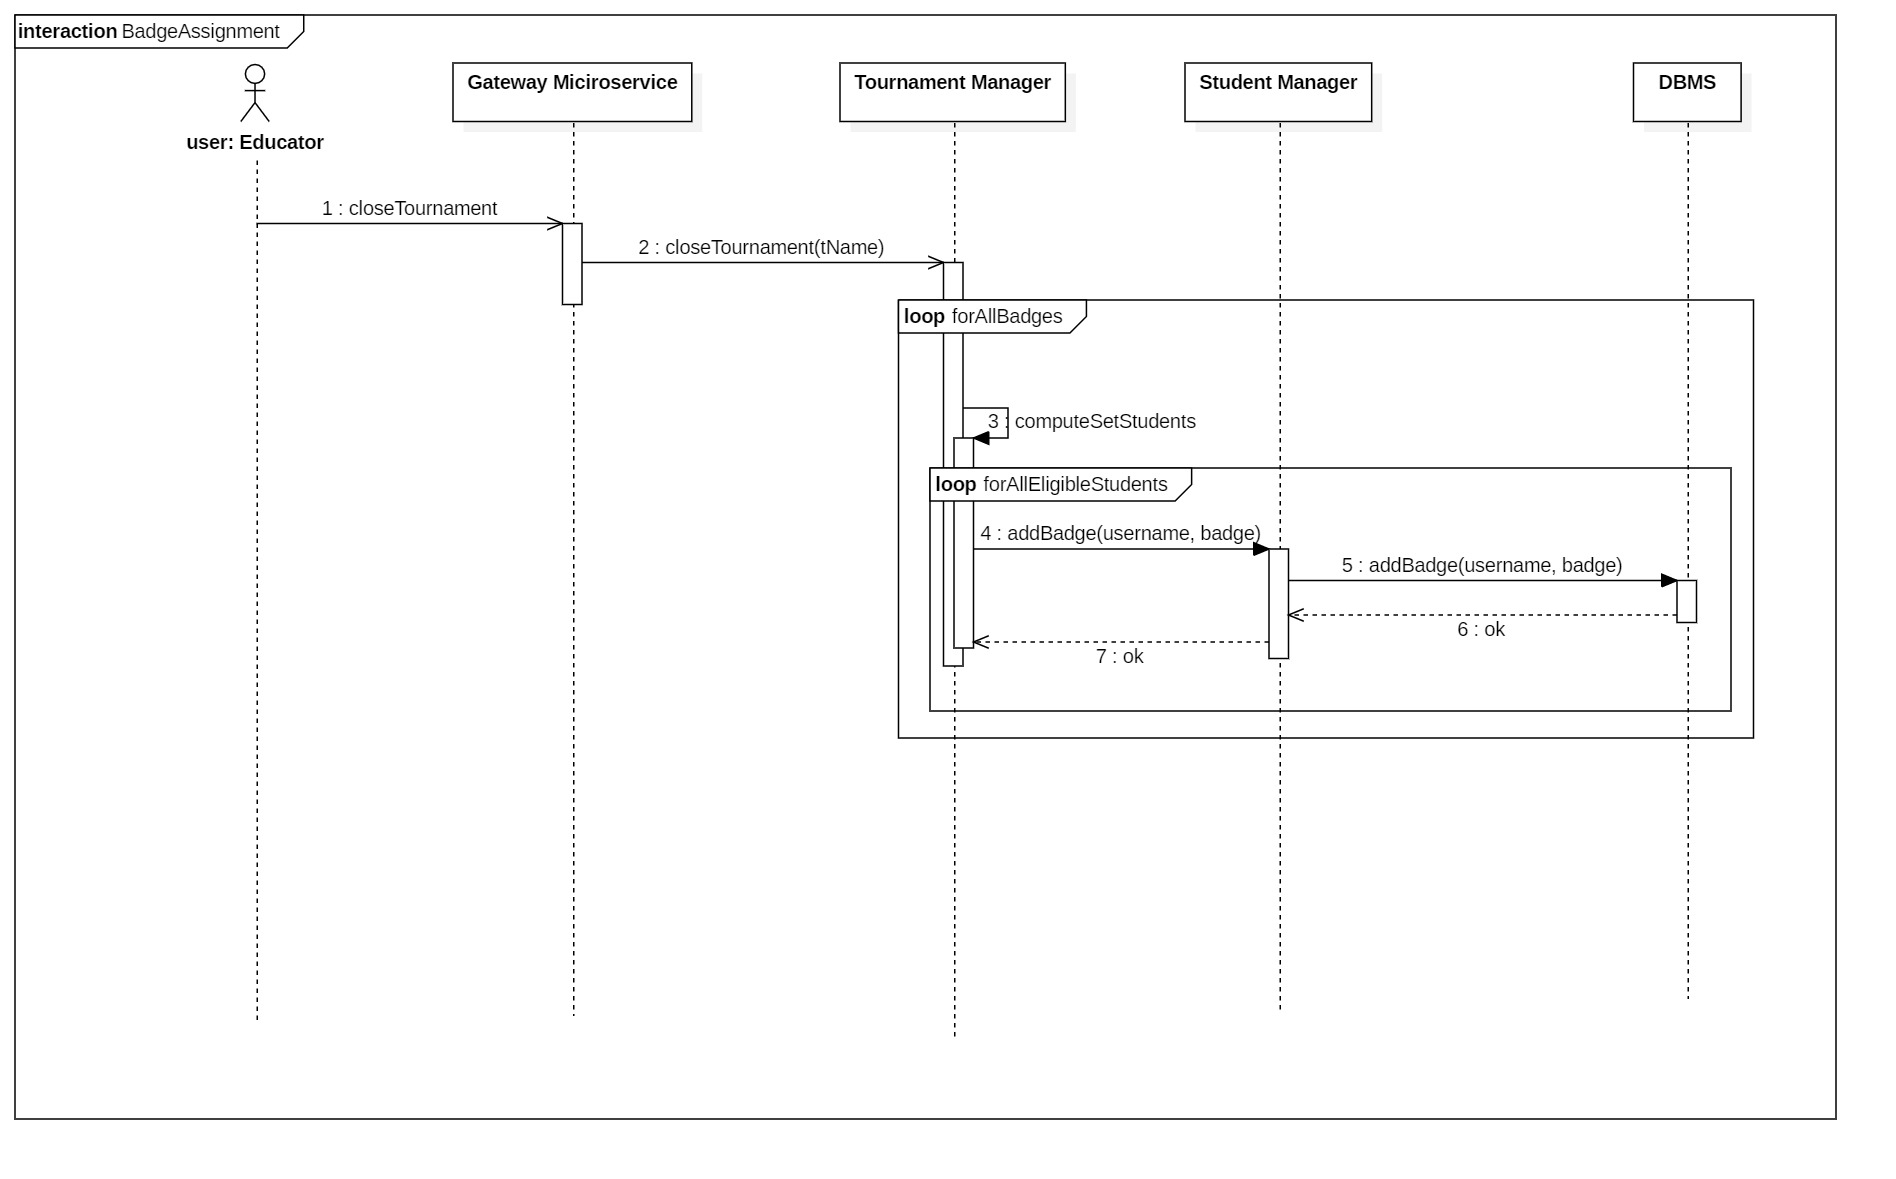
\includegraphics[width=1.3\linewidth, angle=90]{2.ArchitecturalDesign/res/BadgeAssignment.jpg}
    \caption{Runtime view of the assignment of badges}
    \label{fig:badge}
\end{figure}

The sequence starts with the closure of a tournament (see Figure \ref{fig:tournament_end}). Following the closure, the Tournament Manager calculates all the badges to be assigned to the respective teams and, consequently, to the individual students. The loop in the diagram illustrates the process of sending these badges and saving the corresponding data in the DBMS by the Student Manager.

\newpage

\subsubsection*{Code Push}
\begin{figure}[h!]
    \centering
    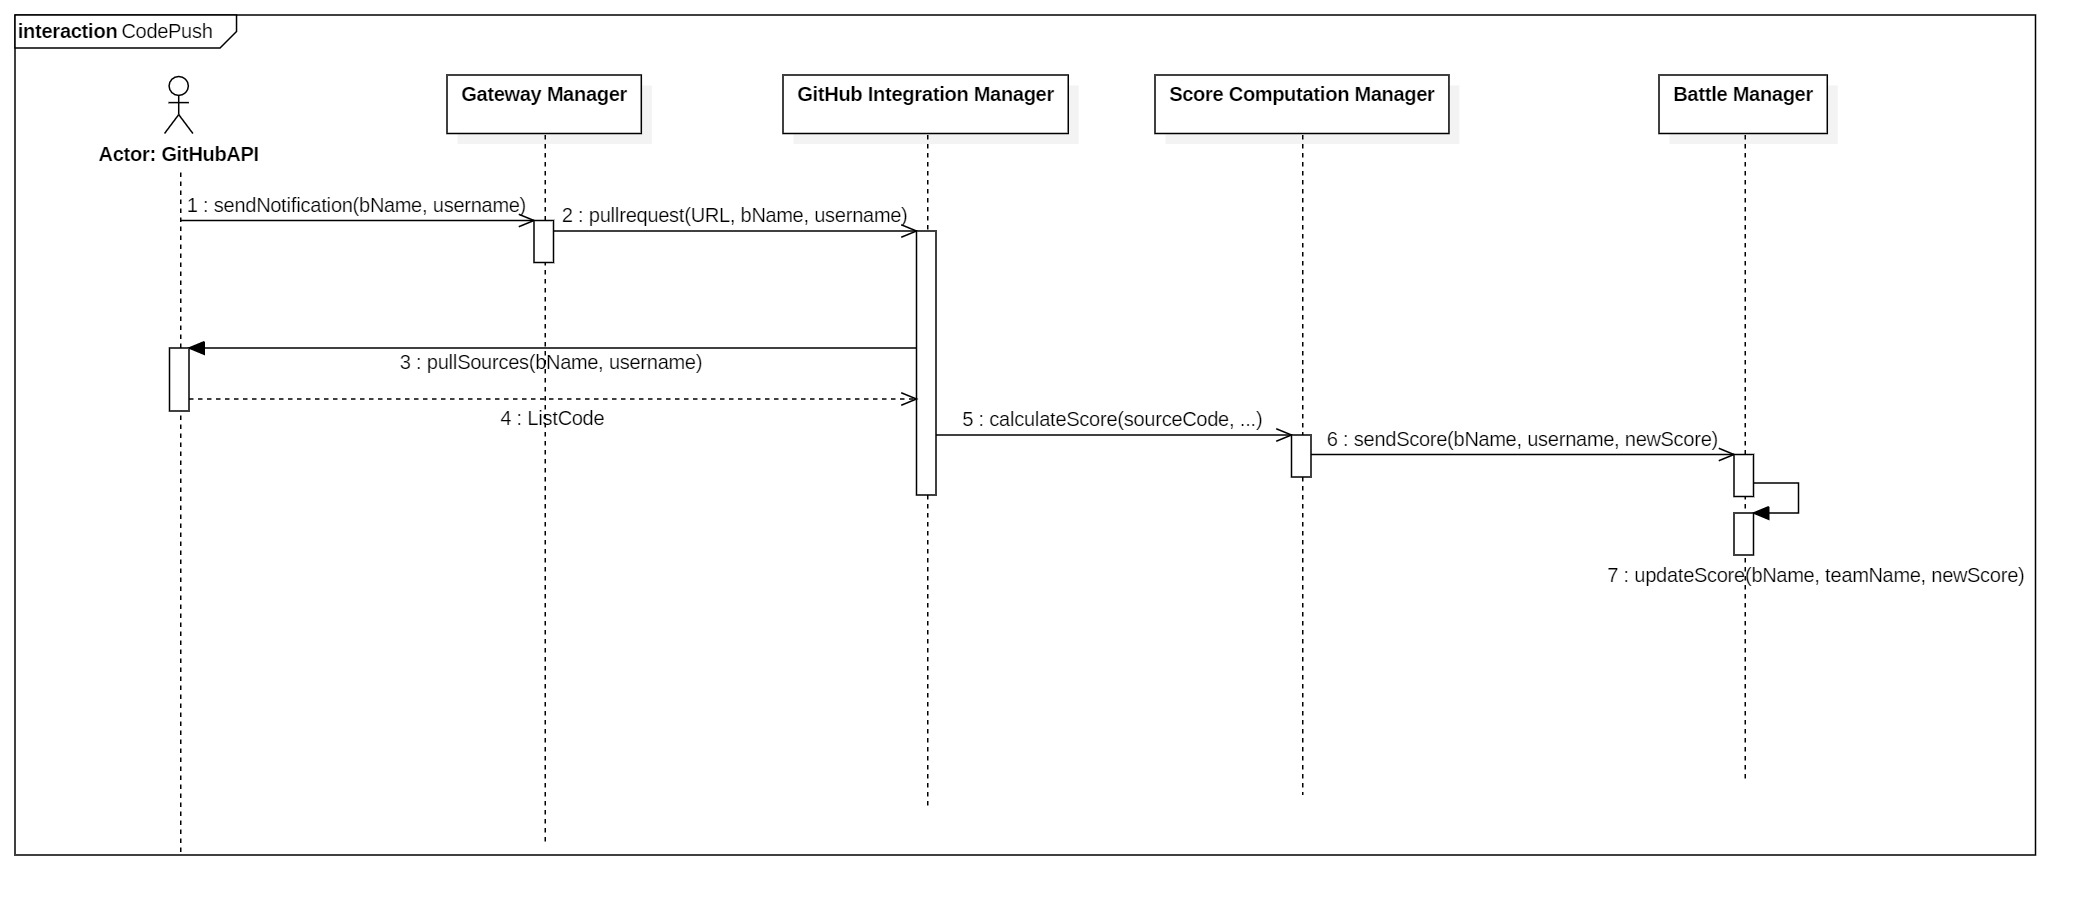
\includegraphics[width=1.3\linewidth, angle=90]{2.ArchitecturalDesign/res/CodePush.jpg}
    \caption{Runtime view when a student pushes the code}
    \label{fig:push}
\end{figure}

The process begins with the action of pushing code, initiated by receiving a notification from the GitHub API indicating that code has been pushed. This notification is received by the Gateway Manager, which then contacts the GitHub Integration Manager to request a pull of the code. The method parameters include the repository URL, the battle name, and the student's username who pushed the code.
Subsequently, the GitHub Integration Manager requests the GitHub API to pull the source code, resulting in a list of code documents that are essential for calculating scores. Following this, the GitHub Integration Manager asks the Score Computation Manager to compute scores, considering various factors such as source code quality, build scripts, test cases, elapsed time, and evaluation criteria.
After calculating the scores, the Score Computation Manager sends the results to the Battle Manager, which updates the local scores accordingly.

\newpage

\subsubsection*{Repository Creation}
\begin{figure}[h!]
    \centering
    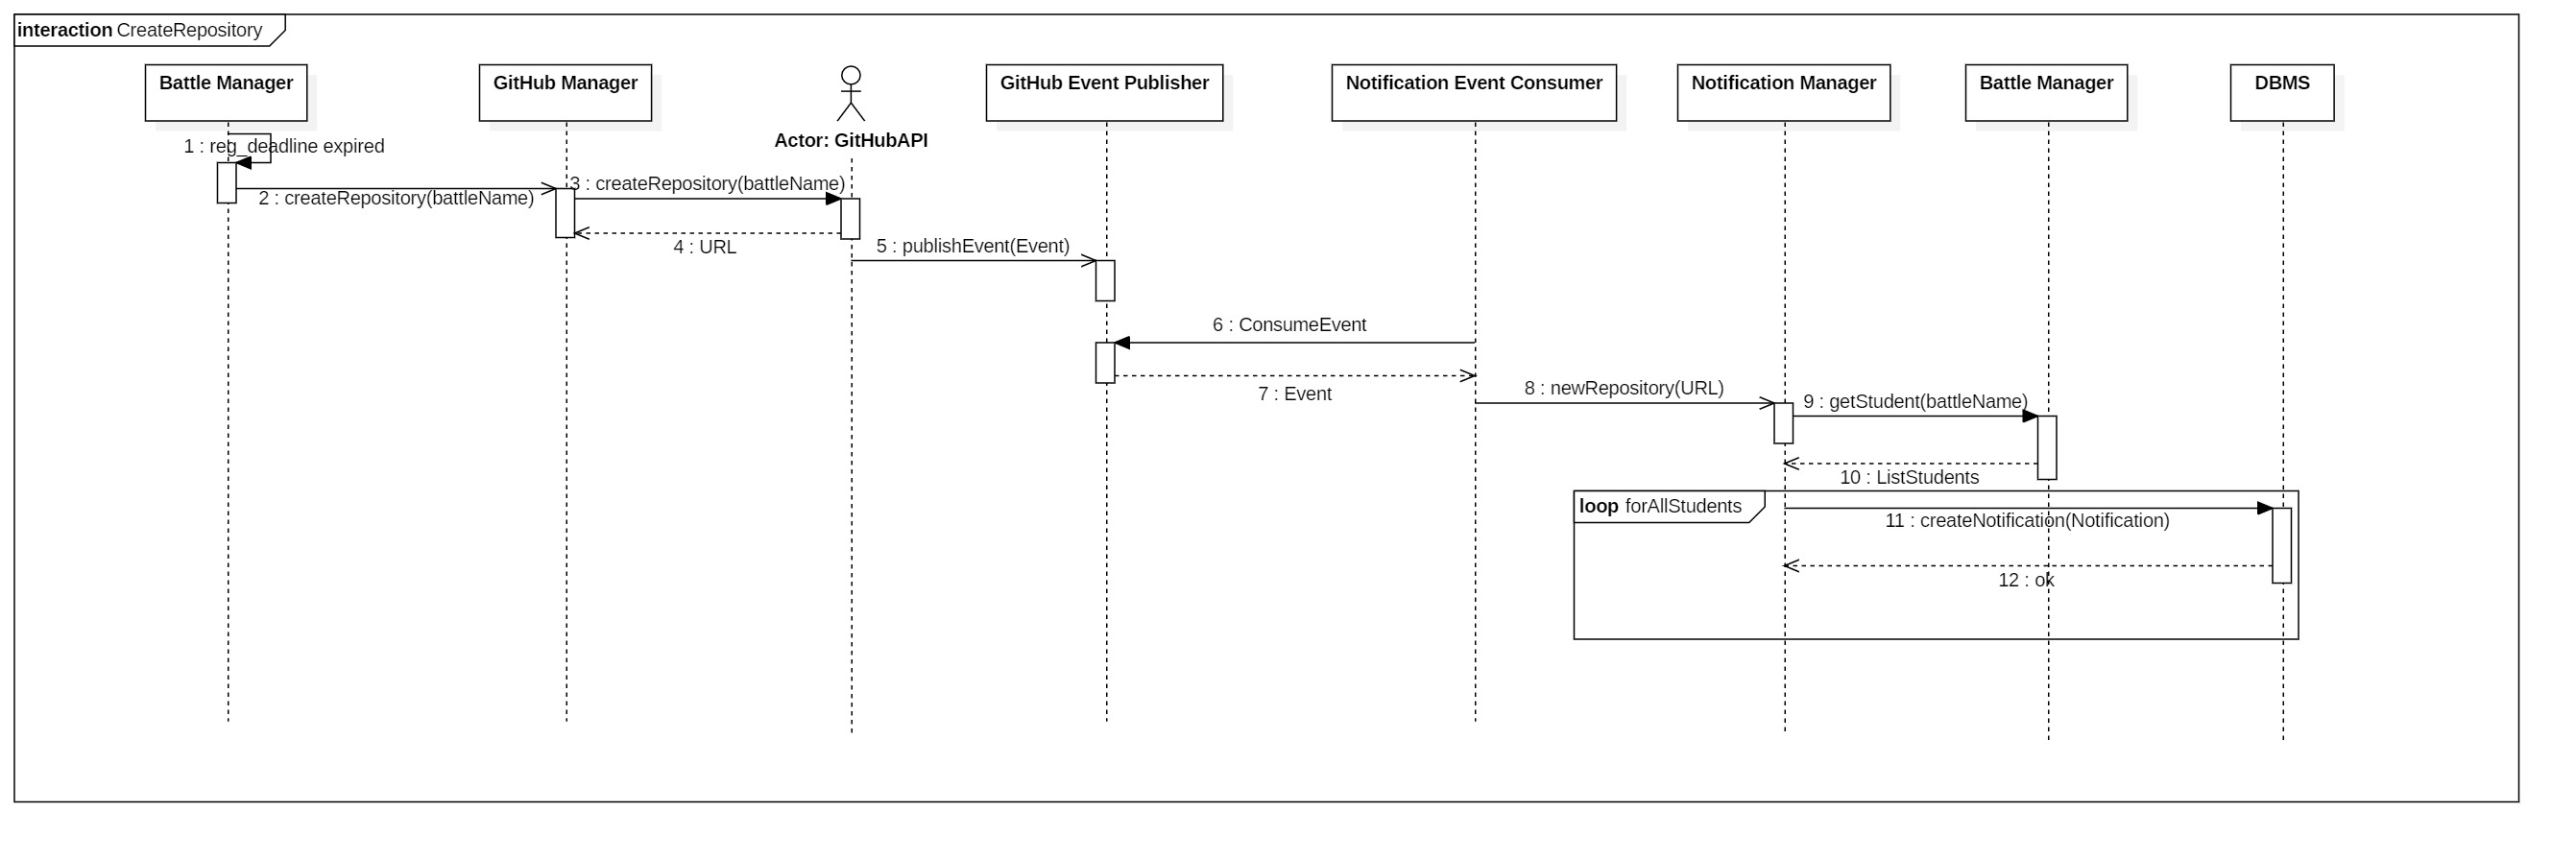
\includegraphics[width=1.3\linewidth, angle=90]{2.ArchitecturalDesign/res/CreateRepository.jpg}
    \caption{Runtime view for creating a repository}
    \label{fig:create_repo}
\end{figure}

The process begins when the Battle Manager detects that the registration deadline for a battle has expired. Following this event, the Battle Manager sends a request to the GitHub Manager to create a new repository for that battle. The GitHub Manager forwards this request to the GitHubAPI, which responds by providing the URL of the newly created repository.
Upon receiving this information, the GitHub Manager publishes a new Event for the Notification Consumer. Subsequently, the Notification Consumer sends notifications to all the students participating in that battle, creating them as described before.

\newpage
\subsubsection*{Score Computation}
\begin{figure}[h!]
    \centering
    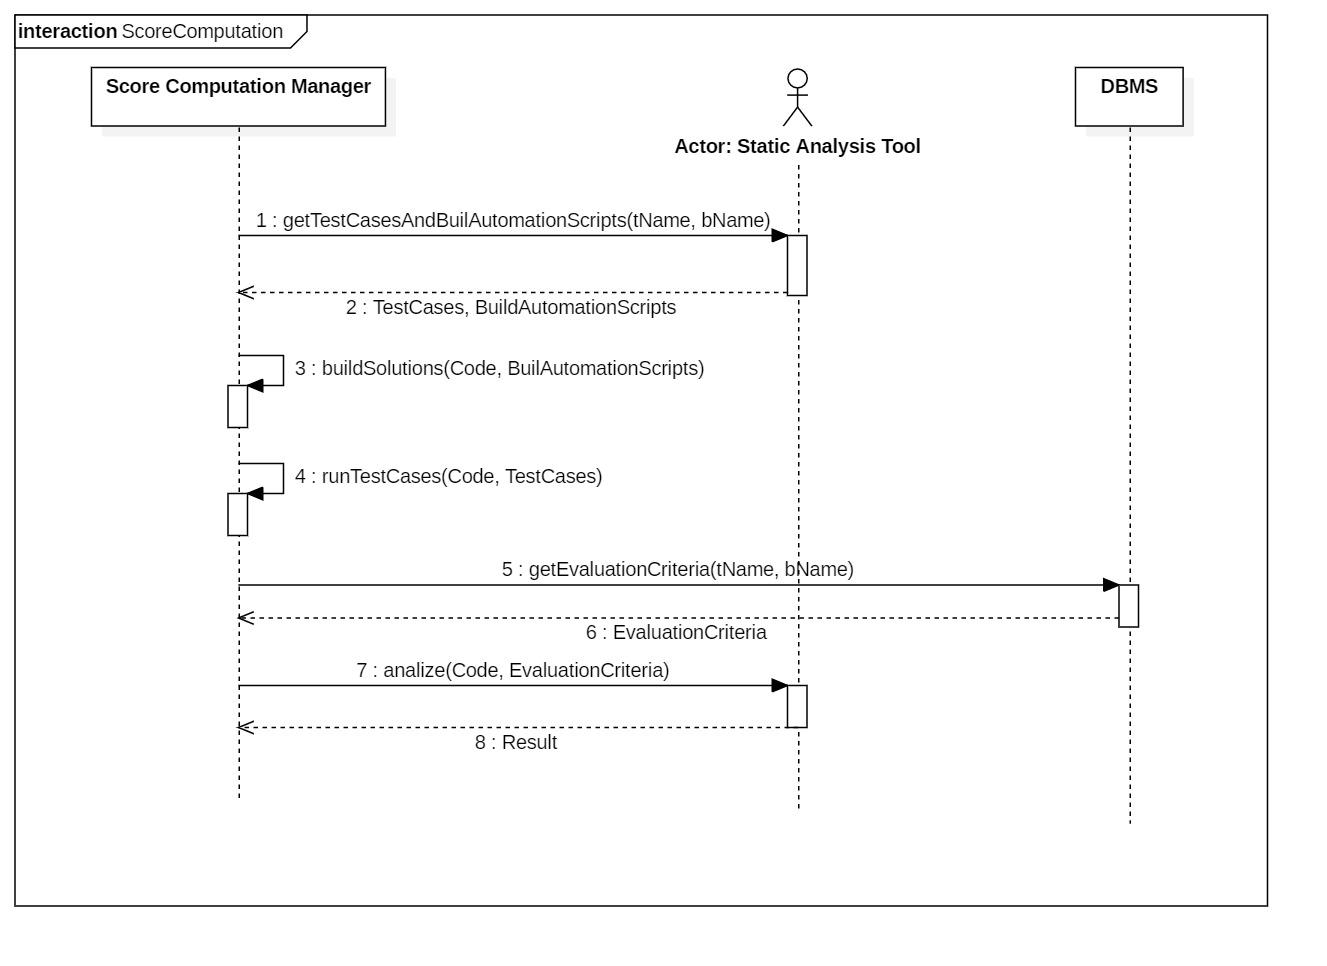
\includegraphics[width=1.3\linewidth]{2.ArchitecturalDesign/res/ScoreComputation.jpg}
    \caption{Runtime view for computing the codes pushed}
    \label{fig:create_repo}
\end{figure}

The process involves two main components, supplemented by an actor: the Score Computation Manager, the Database Management System (DBMS), and the Static Analysis Tool, respectively. To begin the procedure, the Score Computation Manager requests the DBMS to retrieve test cases and generate automation scripts for a specific battle, identified by the bName, within a tournament identified by the tName. Subsequently, it calculates the scores upon constructing the solutions. After that, it queries the DBMS in order to retrieve the evaluation criteria of the same battle. Following this, the Score Computation Manager engages the Static Analysis Tool to analyze the code based on the specified criteria, yielding a conclusive result.


\newpage



\subsection{Component Interfaces}
This section illustrates a comprehensive list of interfaces offered by the various components of the \app system, along with the specifications for their internal methods. A description is provided for each method in order to understand what it is useful for.

The following tables are divided by microservice.

\renewcommand{\arraystretch}{2.3}
\setlength{\tabcolsep}{0.7cm}

\vspace{0.5cm}


% GATEWAY MICROSERVICE -------------------------------------------------------
\begin{large}\textbf{1 - Gateway Microservice}\end{large}\\
\begin{longtable}{|p{2.5cm} p{6.5cm} p{4.5cm}|}
\caption*{DiscoveryServiceI}\\ 

\hline
\textbf{Return Type} & \textbf{Signature} & \textbf{Description}\\
\hline \endhead

URL & findService(String serviceName) & This method is offered to allow all microservices to locate each other and therefore collaborate.\\

void & registerService(String serviceName, URL location) & This method allows a newly-created service to register itself on the list of available services, in order to be located by the other microservices if needed.\\

 List\textless URL\textgreater & allServices() & This method returns a list of all the available services at the moment in the system.\\
 \hline

\end{longtable}


\pagebreak



% USER MANAGEMENT MICROSERVICE ---------------------------------------------
\begin{large}{\textbf{2 - User Management Microservice}}\end{large}\\
The following interfaces are RESTful APIs offered by the Manager components that handle Students and Educators' data.

\begin{longtable}{|p{2.5cm} p{6.5cm} p{4.5cm}|}
	\caption*{StudentAPI}\\ 
	
	\hline
	\textbf{Return Type} & \textbf{Signature} & \textbf{Description}\\
	\hline \endhead
	
	List\textless Student\textgreater & getAllStudents() & This method is offered to retrieve a list of all the students with an account on CodeKataBattle.\\
	
	void & addStudent(username) & Adds a new student the first time it accesses CodeKataBattle. \\
	
	void & removeStudent(username) & Removes the student profile with the specified username from the system.\\
	
	List\textless String\textgreater & getStudentInfo(username) & Retrieves all the information related to a specific student, like list of badges, statistics...\\
	
	List\textless String\textgreater & getBadges(username) & Returns the list of badges won by the student with the specified username.\\
	
	List\textless File\textgreater & getStudentProfileUI(username) & This method builds and returns the files that are needed to offer the user interface for a student's profile.\\
	\hline
	
\end{longtable}

\begin{longtable}{|p{2.5cm} p{6.5cm} p{4.5cm}|}
	\caption*{EducatorAPI}\\ 
	
	\hline
	\textbf{Return Type} & \textbf{Signature} & \textbf{Description}\\
	\hline \endhead
	
	List\textless Educator\textgreater & getAllEducators() & This method is offered to retrieve a list of all the educators with an account on CodeKataBattle.\\
	
	void & addEducator(username) & Adds a new educator the first time it accesses CodeKataBattle. \\
	
	void & removeEducator(username) & Removes the educator profile with the specified username from the system.\\
	
	List\textless File\textgreater & getEducatorProfileUI(username) & This method builds and returns the files that are needed to offer the user interface for an educator's profile.\\
	\hline
	
\end{longtable}

\pagebreak

% TOURNAMENT MICROSERVICE ------------------------------------------
	\begin{large}{\textbf{3 - Tournament Microservice}}\end{large}\\
	The following interface is a RESTful APIs offered by the Manager component that handles Tournaments' data.
	
	\begin{longtable}{|p{2.5cm} p{6.5cm} p{4.5cm}|}
		\caption*{TournamentAPI}\\ 
		
		\hline
		\textbf{Return Type} & \textbf{Signature} & \textbf{Description}\\
		\hline \endhead
		
		void & addTournament(tournamentName, tournamentInfo) & Adds a new tournament to the ones available on the \app platform. Notice that tournamentInfo is a complex entity that comprises a set of mandatory elements for the creation of a new tournament. Tournament names are the identifiers for battles and have to be unique in \app.\\
		
		void & closeTournament (tournamentName) & Closes the tournament with the tournamentName specified. The tournament ranking is published and badges assigned.\\
		
		List\textless Tournament\textgreater & getAllTournaments() & Retrieves a list of all the tournaments available on the \app system in the moment the method is called.\\
		
		void & grantPermissions (tournamentName, username) & This method allows to grant permissions to publish battles to an educator with the specified username in the tournament identified by the tournamentId.\\
		
		void & addStudent(tournamentName, username) & Adds the student with the specified username to the list of students that are subscribed to the tournament.\\
		
		List\textless Student\textgreater & getStudents(tournamentName) & Retrieves a list of all the students that are subscribed to the tournament with the tournamentName specified.\\
		
		List\textless Educator\textgreater & getEducators(tournamentName) & Retrieves a list of all the educators that have permissions to publish battles inside the tournament with the tournamentName specified.\\
		
		String & getCreator(tournamentName) & Returns the username of the Educator that created the tournament with the tournamentName specified.\\
		
		List\textless Badge\textgreater & getBadges(tournamentName) & Retrieves a list of all the badges that have been defined for the tournament with the tournamentName specified.\\
		
		List\textless Float\textgreater & getRanking(tournamentName) & Retrieves the ranking of all students subscribed to a specific tournament with the tournamentName specified.\\
		
		void & updateRanking(tournamentName) & Requires to update the ranking of a tournament with new data that is now available. \\
		
		List\textless Battle\textgreater & getBattles(tournamentName) & Retrieves a list of all the battles that have been published in the tournament with the tournamentName specified.\\
		
		List\textless File\textgreater & getTournamentCreationForm() & Returns all the necessary material to display to an educator the user interface to insert data for a new tournament to be created.\\
			
		List\textless File\textgreater & getTournamentHomePage(tournamentName) & Returns all the necessary material to display to an user of \app the home page of a tournament, with all the information related to it.\\
		
		\hline
		
	\end{longtable}


	\begin{longtable}{|p{2.5cm} p{6.5cm} p{4.5cm}|}
	\caption*{Tournament - EventPublisherI}\\ 
	
	\hline
	\textbf{Return Type} & \textbf{Signature} & \textbf{Description}\\
	\hline \endhead
	
	void & publishEvent(Event)  & Publishes an event on the event bus.\\

	\hline
	
\end{longtable}


	\begin{longtable}{|p{2.5cm} p{6.5cm} p{4.5cm}|}
	\caption*{Tournament - EventConsumerI}\\ 
	
	\hline
	\textbf{Return Type} & \textbf{Signature} & \textbf{Description}\\
	\hline \endhead
	
	Event & consumeEvent()  & Reads an event from the event bus.\\
	
	List\textless Event\textgreater & consumeAllEvents() & Reads all the events published on the event bus.\\
	
	\hline
	
\end{longtable}

\pagebreak



%BATTLE MICROSERVICE ---------------------------------------------------
\begin{large}{\textbf{4 - Battle Microservice}}\end{large}\\
The following interface is a RESTful APIs offered by the Manager component that handles Battles' data.
\begin{longtable}{|p{2.5cm} p{6.5cm} p{4.5cm}|}
	\caption*{BattleAPI}\\ 
	
	\hline
	\textbf{Return Type} & \textbf{Signature} & \textbf{Description}\\
	\hline \endhead
	
	void & addBattle(battleName, tournamentName, battleInfo) & Adds a new battle to the tournament specified with tournamentName. Notice that battleInfo is a complex entity that comprises a set of mandatory elements for the creation of a new battle. Battle names are the identifiers for battles and have to be unique in \app.\\
	
	void & terminateBattle(battleName) & Terminates the battle named battleName; the final ranking is drawn and published.\\
	
	void & addTeam(battleName, teamName, List\textless Student\textgreater) & Adds a new team to the battle called battleName, composed of the students specified in the second parameter of the function. In case of a single student, the teamName is the username of the solo player by default.\\
	
	String & getCreator(battleName) & Returns the username of the educator that created the battle named battleName.\\
	
	List\textless Team\textgreater & getAllTeams(battleName) & Retrieves a list of all the teams that participate in the battle named battleName.\\
	
	List\textless Student\textgreater & getAllStudents(battleName) & Retrieves a list of all the students participating in the battle named battleName.\\
	
	List\textless Student\textgreater & getStudentsInTeam(battleName, teamName) & Retrieves a list of usernames of the students that are part of a specific team named teamName inside the battle battleName.\\
	
	List\textless Float\textgreater & getRanking(battleName) & Retrieves the ranking of the battle named battleName.\\
	
	void & updateScore(battleName, teamName, newScore) & Updates the maximum score assigned to a specific team and the ranking is changed accordingly.\\
	
	Float & getTeamScore(battleName, teamName) & Retrieves the maximum score assigned to a team in a battle so far.\\
	
	Date & getCreationTime(battleName) & Returns the exact date and time when the battle called battleName was created (useful for computing scores).\\
	
	List\textless File\textgreater & getBattleCreationForm() & Returns all the necessary material to display to an educator the user interface to insert data for a new battle to be created.\\
	
	List\textless File\textgreater & getTournamentHomePage(battleName) & Returns all the necessary material to display to an user the home page of the battle named battleName.\\
	
	\hline
	
\end{longtable}




\begin{longtable}{|p{2.5cm} p{6.5cm} p{4.5cm}|}
\caption*{Battle - EventPublisherI}\\ 

\hline
\textbf{Return Type} & \textbf{Signature} & \textbf{Description}\\
\hline \endhead

void & publishEvent(Event)  & Publishes an event on the event bus.\\

\hline

\end{longtable}

\pagebreak


% NOTIFICATION MICROSERVICE ----------------------------------------
\begin{large}{\textbf{5 - Notification Microservice}}\end{large}\\
The following interface is a RESTful APIs offered by the Manager component that handles Notification data.
\begin{longtable}{|p{2.5cm} p{6.5cm} p{4.5cm}|}
	\caption*{NotificationAPI}\\ 
	
	\hline
	\textbf{Return Type} & \textbf{Signature} & \textbf{Description}\\
	\hline \endhead
	
	List\textless Notification\textgreater & getNotifications(username) & Retrieves all the notifications that are stored for the user with the specified username.\\
	
	List\textless File\textgreater & getNotificationUI() & Returns all the necessary material to display to a student the user interface to see the notifications that have arrived to him/her on CodeKataBattle.\\
	
	\hline
	
\end{longtable}




\begin{longtable}{|p{2.5cm} p{6.5cm} p{4.5cm}|}
	\caption*{Notification - EventConsumerI}\\ 
	
	\hline
	\textbf{Return Type} & \textbf{Signature} & \textbf{Description}\\
	\hline \endhead
	
	Event & consumeEvent()  & Reads an event from the event bus.\\
	
	List\textless Event\textgreater & consumeAllEvents() & Reads all the events published on the event bus.\\
	
	\hline
	
\end{longtable}


\pagebreak

% GITHUB INTEGRATION MICROSERVICE ----------------------------------------
\begin{large}{\textbf{6 - GitHub Integration Microservice}}\end{large}\\
The following interface is a RESTful APIs offered by the Manager component that handles GitHub integration with CodeKataBattle.
\begin{longtable}{|p{2.5cm} p{6.5cm} p{4.5cm}|}
	\caption*{GitHubIntegrationAPI}\\ 
	
	\hline
	\textbf{Return Type} & \textbf{Signature} & \textbf{Description}\\
	\hline \endhead
	
	URL & getRepositoryLink(battleName) & Retrieves the link to the remote GitHub repository created by \app for the battle named battleName.\\
	
	URL & createRepository(battleName) & Creates a new GitHub repository for the battle named battleName and returns its link.\\
	
	void & removeRepository(battleName) & Deletes the GitHub repository for the battle named battleName, when the battle is closed.\\
	
	void & newCommit(battleName, username) & This method is offered to receive notifications from GitHub when a new commit is performed by a student in a repository that stores solutions for a battle named battleName.\\
	
	List\textless File\textgreater & pullSources(battleName, username) &  Downloads the latest source code files for the user specified by username in the context of the battle named battleName.\\
	
	\hline
	
\end{longtable}

\begin{longtable}{|p{2.5cm} p{6.5cm} p{4.5cm}|}
	\caption*{GitHub Integration - EventConsumerI}\\ 
	
	\hline
	\textbf{Return Type} & \textbf{Signature} & \textbf{Description}\\
	\hline \endhead
	
	Event & consumeEvent()  & Reads an event from the event bus.\\
	
	List\textless Event\textgreater & consumeAllEvents() & Reads all the events published on the event bus.\\
	
	\hline
	
\end{longtable}

\vspace{1cm}

\begin{large}{\textbf{7 - Score Computation Microservice}}\end{large}\\

\begin{longtable}{|p{2.5cm} p{6.5cm} p{4.5cm}|}
	\caption*{CalculatorAPI}\\ 
	
	\hline
	\textbf{Return Type} & \textbf{Signature} & \textbf{Description}\\
	\hline \endhead
	
	Float & calculateScore(sourceCode, buildScripts, testCases, timePassed, evaluationCriteria) & This method implements the main functionality of the microservice, which is computing the score of a specific solution submitted by a student and return it.\\
	
	\hline
	
\end{longtable}

\subsection{Selected Architectural Styles and Patterns}
\subsection{Other Design Decisions}